%% 
%% Copyright 2007-2024 Elsevier Ltd
%% 
%% This file is part of the 'Elsarticle Bundle'.
%% ---------------------------------------------
%% 
%% It may be distributed under the conditions of the LaTeX Project Public
%% License, either version 1.3 of this license or (at your option) any
%% later version.  The latest version of this license is in
%%    http://www.latex-project.org/lppl.txt
%% and version 1.3 or later is part of all distributions of LaTeX
%% version 1999/12/01 or later.
%% 
%% The list of all files belonging to the 'Elsarticle Bundle' is
%% given in the file `manifest.txt'.
%% 
%% Template article for Elsevier's document class `elsarticle'
%% with numbered style bibliographic references
%% SP 2008/03/01
%% $Id: elsarticle-template-num.tex 249 2024-04-06 10:51:24Z rishi $
%%
\documentclass[preprint,12pt]{elsarticle}
% Allow inclusion of PDF 1.7 figures without version mismatch warnings
\pdfminorversion=7

%% Use the option review to obtain double line spacing
%% \documentclass[authoryear,preprint,review,12pt]{elsarticle}

%% Use the options 1p,twocolumn; 3p; 3p,twocolumn; 5p; or 5p,twocolumn
%% for a journal layout:
%% \documentclass[final,1p,times]{elsarticle}
%% \documentclass[final,1p,times,twocolumn]{elsarticle}
%% \documentclass[final,3p,times]{elsarticle}
%% \documentclass[final,3p,times,twocolumn]{elsarticle}
%% \documentclass[final,5p,times]{elsarticle}
%% \documentclass[final,5p,times,twocolumn]{elsarticle}

%% For including figures, graphicx.sty has been loaded in
%% elsarticle.cls. If you prefer to use the old commands
%% please give \usepackage{epsfig}

%% The amssymb package provides various useful mathematical symbols
% \usepackage{cite}
\usepackage{amsmath,amssymb,amsfonts}
% \usepackage{algorithmic}
\usepackage[ruled,vlined]{algorithm2e}
\usepackage{graphicx}
% \usepackage{algorithm,algorithmic}
\usepackage{hyperref}
% \usepackage[numbers,sort&compress]{natbib}
\usepackage[caption=false,font=footnotesize,labelfont=sf,textfont=sf]{subfig}
\usepackage{array}
\usepackage{balance}
% \usepackage{enumitem}       % For customizable lists (conflicts with IEEEtran)
\usepackage{booktabs}       % For professional tables with \toprule, \midrule, etc.
\usepackage{multirow}       % For table cells spanning multiple rows
\usepackage{makecell}       % For better table cell formatting
\usepackage{tikz}           % For flowcharts or block diagrams
\usetikzlibrary{shapes,arrows.meta,positioning,calc,shadows,backgrounds,decorations.pathreplacing,fit,petri,arrows}

% Hyperref setup: colored citations and links, enable Unicode, and safer PDF string handling
\hypersetup{
  colorlinks=true,
  linkcolor=blue,
  citecolor=blue,
  urlcolor=blue,
  unicode=true,
  pdfencoding=auto,
  psdextra
}
% Disable/neutralize commands that can appear in PDF strings (titles, bookmarks)
\pdfstringdefDisableCommands{%
  \def\thanks#1{}%
  \def\footnote#1{}%
  \def\cortext#1{}%
}
\usepackage{textcomp}
%% \usepackage{amsthm}

%% The lineno packages adds line numbers. Start line numbering with
%% \begin{linenumbers}, end it with \end{linenumbers}. Or switch it on
%% for the whole article with \linenumbers.
%% \usepackage{lineno}

% \journal{Computer Methods and Programs in Biomedicine}
\journal{Artificial Intelligence in Medicine}

\begin{document}

\begin{frontmatter}

%% Title, authors and addresses

%% use the tnoteref command within \title for footnotes;
%% use the tnotetext command for theassociated footnote;
%% use the fnref command within \author or \affiliation for footnotes;
%% use the fntext command for theassociated footnote;
%% use the corref command within \author for corresponding author footnotes;
%% use the cortext command for theassociated footnote;
%% use the ead command for the email address,
%% and the form \ead[url] for the home page:
%% \title{Title\tnoteref{label1}}
%% \tnotetext[label1]{}
%% \author{Name\corref{cor1}\fnref{label2}}
%% \ead{email address}
%% \ead[url]{home page}
%% \fntext[label2]{}
%% \cortext[cor1]{}
%% \affiliation{organization={},
%%             addressline={},
%%             city={},
%%             postcode={},
%%             state={},
%%             country={}}
%% \fntext[label3]{}

% \title{MSAGAT-Net: An Efficient Multi-Scale Temporal Graph Attention Network for Spatiotemporal Epidemic Forecasting}

\title{MSAGAT-Net: Multi-Scale Adaptive Graph Attention Network for Efficient Spatiotemporal Epidemic Forecasting}

%% use optional labels to link authors explicitly to addresses:
%% \author[label1,label2]{}
%% \affiliation[label1]{organization={},
%%             addressline={},
%%             city={},
%%             postcode={},
%%             state={},
%%             country={}}
%%
%% \affiliation[label2]{organization={},
%%             addressline={},
%%             city={},
%%             postcode={},
%%             state={},
%%             country={}}

% Authors and affiliations
% --- Authors ---
\author[inst1]{Michael Ajao-olarinoye\corref{cor1}\fnref{fn1}}
\ead{olarinoyem@coventry.ac.uk}

\author[inst1]{Vasile Palade\fnref{fn1}}
\author[inst1]{Fei He}
\author[inst2]{Petra A Wark}
\author[inst1]{Seyed Mousavi}
\author[inst3]{Zindoga Mukandavire}

% --- Notes & correspondence ---
\cortext[cor1]{Corresponding author.}
% \fntext[fn1]{These authors contributed equally to this work.}

% --- Affiliations ---
\affiliation[inst1]{%
  organization={Centre for Computational Science and Mathematical Modelling, Coventry University},
  city={Coventry},
  country={United Kingdom}
}

\affiliation[inst2]{%
  organization={Research Methods and Evaluation Unit, Research Centre for Healthcare and Communities, Coventry University},
  city={Coventry},
  country={United Kingdom}
}

\affiliation[inst3]{%
  organization={Institute of Applied Research and Technology, Emirates Aviation University},
  city={Dubai},
  country={United Arab Emirates}
}
\begin{abstract}
\textbf{Background and Objective:} Graph neural networks for spatiotemporal epidemic forecasting face three computational limitations: mandatory reliance on predefined adjacency matrices, lack of adaptive control over how structural priors influence learned attention across different graph densities, and unstable multi-horizon predictions. We introduce MSAGAT-Net, a multi-scale adaptive graph attention network that addresses these limitations through novel computational mechanisms.

\textbf{Methods:} The central methodological contribution is a \emph{self-regulating additive structural bias} in graph attention: a learnable low-rank graph bias and an optional adjacency prior are added directly to attention scores before softmax normalisation, where softmax shift-invariance causes the prior's influence to adapt automatically---negligible on dense graphs, meaningful on sparse ones---eliminating fragile graph-size-dependent thresholds. A second contribution is an adaptive multi-hop spatial module whose diffusion depth scales with graph size to prevent oversmoothing on small graphs. These core mechanisms are supported by depthwise separable temporal feature extraction, progressive prediction refinement with a learnable decay rate, and a highway autoregressive connection. Unlike existing baselines, MSAGAT-Net learns spatial relationships entirely from data without requiring predefined adjacency matrices.

\textbf{Results:} Evaluation on six diverse datasets spanning influenza, COVID-19, and ICU bed occupancy shows that MSAGAT-Net achieves the best RMSE in the majority of settings, with improvements of up to 23.5\% on LTLA-Timeseries (372 local authorities) and 22.2\% on NHS-Timeseries over the strongest baselines.

\textbf{Conclusions:} Ablation studies reveal that architectural importance is fundamentally horizon-dependent: adaptive spatial attention is universally essential, while spatial refinement and prediction modules become increasingly important as forecast difficulty increases. These findings demonstrate the value of self-regulating computational mechanisms for graph-based biomedical forecasting.
\end{abstract}


% %%Graphical abstract
% \begin{graphicalabstract}
% %\includegraphics{grabs}
% \end{graphicalabstract}

%%Research highlights
\begin{highlights}
\item Self-regulating graph attention adapts to any graph density
\item Adjacency-free spatial learning needs no predefined graph
\item Adaptive multi-hop convolutions prevent oversmoothing
\item Up to 23.5\% RMSE reduction on 372-region COVID-19 data
\item Ablation reveals horizon-dependent component importance
\end{highlights}

%% Keywords
\begin{keyword}
% %% keywords here, in the form: keyword \sep keyword

% %% PACS codes here, in the form: \PACS code \sep code

% %% MSC codes here, in the form: \MSC code \sep code
% %% or \MSC[2008] code \sep code (2000 is the default)
%   (old keywords removed)
Graph neural networks \sep self-regulating attention \sep adaptive graph learning \sep epidemic forecasting \sep spatiotemporal forecasting \sep multi-scale modelling
\end{keyword}



\end{frontmatter}

%% Add \usepackage{lineno} before \begin{document} and uncomment 
%% following line to enable line numbers
%% \linenumbers

%% main text
%%

%% Use \section commands to start a section
% \section{Example Section}
% \label{sec1}
% %% Labels are used to cross-reference an item using \ref command.

% Section text. See Subsection \ref{subsec1}.

% %% Use \subsection commands to start a subsection.
% \subsection{Example Subsection}
% \label{subsec1}

% Subsection text.

% %% Use \subsubsection, \paragraph, \subparagraph commands to 
% %% start 3rd, 4th and 5th level sections.
% %% Refer following link for more details.
% %% https://en.wikibooks.org/wiki/LaTeX/Document_Structure#Sectioning_commands

% \subsubsection{Mathematics}
% %% Inline mathematics is tagged between $ symbols.
% This is an example for the symbol $\alpha$ tagged as inline mathematics.

% %% Displayed equations can be tagged using various environments. 
% %% Single line equations can be tagged using the equation environment.
% \begin{equation}
% f(x) = (x+a)(x+b)
% \end{equation}

% %% Unnumbered equations are tagged using starred versions of the environment.
% %% amsmath package needs to be loaded for the starred version of equation environment.
% \begin{equation*}
% f(x) = (x+a)(x+b)
% \end{equation*}

% %% align or eqnarray environments can be used for multi line equations.
% %% & is used to mark alignment points in equations.
% %% \\ is used to end a row in a multiline equation.
% \begin{align}
%  f(x) &= (x+a)(x+b) \\
%       &= x^2 + (a+b)x + ab
% \end{align}

% \begin{eqnarray}
%  f(x) &=& (x+a)(x+b) \nonumber\\ %% If equation numbering is not needed for a row use \nonumber.
%       &=& x^2 + (a+b)x + ab
% \end{eqnarray}

% %% Unnumbered versions of align and eqnarray
% \begin{align*}
%  f(x) &= (x+a)(x+b) \\
%       &= x^2 + (a+b)x + ab
% \end{align*}

% \begin{eqnarray*}
%  f(x)&=& (x+a)(x+b) \\
%      &=& x^2 + (a+b)x + ab
% \end{eqnarray*}

% %% Refer following link for more details.
% %% https://en.wikibooks.org/wiki/LaTeX/Mathematics
% %% https://en.wikibooks.org/wiki/LaTeX/Advanced_Mathematics

% %% Use a table environment to create tables.
% %% Refer following link for more details.
% %% https://en.wikibooks.org/wiki/LaTeX/Tables
% \begin{table}[t]%% placement specifier
% %% Use tabular environment to tag the tabular data.
% %% https://en.wikibooks.org/wiki/LaTeX/Tables#The_tabular_environment
% \centering%% For centre alignment of tabular.
% \begin{tabular}{l c r}%% Table column specifiers
% %% Tabular cells are separated by &
%   1 & 2 & 3 \\ %% A tabular row ends with \\
%   4 & 5 & 6 \\
%   7 & 8 & 9 \\
% \end{tabular}
% %% Use \caption command for table caption and label.
% \caption{Table Caption}\label{fig1}
% \end{table}


% %% Use figure environment to create figures
% %% Refer following link for more details.
% %% https://en.wikibooks.org/wiki/LaTeX/Floats,_Figures_and_Captions
% \begin{figure}[t]%% placement specifier
% %% Use \includegraphics command to insert graphic files. Place graphics files in 
% %% working directory.
% \centering%% For centre alignment of image.
% \includegraphics{example-image-a}
% %% Use \caption command for figure caption and label.
% \caption{Figure Caption}\label{fig1}
% %% https://en.wikibooks.org/wiki/LaTeX/Importing_Graphics#Importing_external_graphics
% \end{figure}


% %% The Appendices part is started with the command \appendix;
% %% appendix sections are then done as normal sections
% \appendix
% \section{Example Appendix Section}
% \label{app1}

% Appendix text.

% %% For citations use: 
% %%       \cite{<label>} ==> [1]

% %%
% Example citation, See \cite{lamport94}.

% %% If you have bib database file and want bibtex to generate the
% %% bibitems, please use
% %%
% %%  \bibliographystyle{elsarticle-num} 
% %%  \bibliography{<your bibdatabase>}

% %% else use the following coding to input the bibitems directly in the
% %% TeX file.

% %% Refer following link for more details about bibliography and citations.
% %% https://en.wikibooks.org/wiki/LaTeX/Bibliography_Management

% \begin{thebibliography}{00}

% %% For numbered reference style
% %% \bibitem{label}
% %% Text of bibliographic item

% \bibitem{lamport94}
%   Leslie Lamport,
%   \textit{\LaTeX: a document preparation system},
%   Addison Wesley, Massachusetts,
%   2nd edition,
%   1994.

% \end{thebibliography}

\section{Introduction}
\label{sec:introduction}
Graph attention mechanisms have become a central computational tool for modelling spatiotemporal dependencies in biomedical data, with applications spanning epidemic forecasting \cite{ajao2023deep, kimForecastingEpidemicSpread2025}, clinical time series prediction, and healthcare resource planning. However, existing graph attention architectures face fundamental computational limitations that restrict their practical deployment: they are typically over-parameterised, mandate predefined adjacency matrices constructed from external data sources, and provide no mechanism to adaptively control how structural priors influence the learned attention across graphs of varying density and size. These are not merely application-specific shortcomings but general deficiencies in the graph attention methodology itself.

These limitations are particularly acute in spatiotemporal epidemic forecasting, where models must capture complex interactions between spatial dependencies (how diseases spread between interconnected regions) and temporal patterns ranging from daily reporting fluctuations to seasonal waves \cite{Panja2022Epicasting, Stone2007Seasonal}. The COVID-19 pandemic has underscored the need for reliable computational methods that can adapt to rapidly changing dynamics across hundreds or thousands of regions \cite{da2021covid, giuliani2020modelling, verma2022temporal, ma2024reporting}, yet traditional epidemiological models struggle with the computational complexity required for real-time surveillance at this scale \cite{heltberg2022spatial, s25082507, DEANGELIS201583}.

Deep learning techniques, originally demonstrated in traffic forecasting \cite{li2017diffusion, zhang2021graph} and environmental monitoring \cite{wu2018deep, lai2018modeling}, have advanced epidemic prediction through recurrent, convolutional, and graph neural network architectures \cite{ajao2023deep, zhiweidingBiologyInformedRecurrentNeural2023, Ahmadini2025, Kamalov2022ReviewDL, wang2019defsi}. Graph neural networks in particular have shown strong potential by learning complex spatiotemporal patterns from data, outperforming traditional models in capturing regional heterogeneity and dynamic transmission mechanisms. Despite these advances, current approaches face four fundamental computational limitations: (1) most graph attention mechanisms are over-parameterised and offer no mechanism to control how much structural prior influences the learned attention, causing performance to vary unpredictably across graphs of different density and size; (2) state-of-the-art models such as EpiGNN, Cola-GNN, and DCRNN require predefined adjacency matrices constructed from geographical proximity or mobility data, which may not capture the true epidemic transmission patterns and require domain expertise or external data sources that may be unavailable; (3) existing methods typically employ fixed architectural choices for spatial processing, failing to adapt to the diverse graph sizes and dynamics exhibited by different diseases and forecast horizons; and (4) multi-horizon forecasting remains unstable due to error accumulation, limiting the utility of long-range forecasts essential for public health planning and resource allocation.

To address these challenges, we propose MSAGAT-Net (Multi-Scale Adaptive Graph Attention Network), a novel architecture whose central contribution is a \emph{self-regulating additive structural bias} in graph attention that automatically adapts to graph density without manual tuning. The architecture comprises two novel modules---an Efficient Adaptive Graph Attention Module (EAGAM) with learnable low-rank graph bias and self-regulating adjacency prior, and a Multi-Scale Spatial Feature Module (MSSFM) with graph-size-adaptive multi-hop convolutions and locality-biased fusion---supported by depthwise separable temporal feature extraction (TFEM), progressive prediction refinement with a learnable decay rate (PPRM), and a highway autoregressive connection.

Our key contributions are as follows:

\begin{enumerate}
    \item \textbf{Self-regulating additive structural bias attention (EAGAM).} We propose a graph attention mechanism that adds a learnable low-rank graph bias and an optional adjacency prior directly to attention scores before softmax normalisation. Softmax shift-invariance causes this additive prior to self-regulate across graph densities---negligible on dense graphs, meaningful on sparse ones---eliminating graph-size-dependent thresholds used in prior work and enabling the model to learn spatial relationships entirely from data. Unlike EpiGNN, Cola-GNN, and DCRNN, MSAGAT-Net does not require predefined adjacency matrices; ablation confirms comparable or better performance without any adjacency input.

    \item \textbf{Adaptive multi-hop spatial refinement with anti-oversmoothing (MSSFM).} We introduce a spatial module that aggregates multi-hop graph convolutions with locality-biased learnable fusion weights and adapts the maximum diffusion depth to graph size, preventing oversmoothing on small graphs while retaining broader spatial context on larger ones. This graph-size-adaptive mechanism is absent from existing epidemic GNNs.

    \item \textbf{Comprehensive evaluation and scientific insights.} We evaluate MSAGAT-Net on six diverse epidemic datasets spanning influenza, COVID-19, and ICU bed occupancy, achieving the best RMSE in the majority of settings, with improvements of up to 23.5\% on LTLA-Timeseries and 22.2\% on NHS-Timeseries over the strongest baselines. Ablation studies reveal that architectural importance is fundamentally horizon-dependent: adaptive spatial attention is universally essential, while spatial refinement and prediction modules become increasingly important as forecast difficulty increases.

\end{enumerate}

The remainder of this paper is organised as follows. Section~\ref{sec:related_work} reviews the literature on spatiotemporal epidemic forecasting, graph neural networks, attention mechanisms, and multi-scale temporal modelling. Section~\ref{sec:methodology} formalises the forecasting problem, describes the data pre-processing and graph construction procedures, and presents the proposed MSAGAT-Net architecture. Section~\ref{sec:experiments} details the experimental setup, datasets, baseline methods, and evaluation metrics. Section~\ref{sec:results} presents a comprehensive comparison of the results, ablation studies of model components, analysis across forecasting horizons, and qualitative visualisations to aid interpretation. Finally, Section~\ref{sec:conclusion} summarises the key findings and contributions, discusses limitations and practical implications for public health decision making, and outlines directions for future research.

% ---------- SECTION II: LITERATURE REVIEW ----------
\section{Related Work}
\label{sec:related_work} 

Epidemic forecasting has evolved from classical compartmental models to neural network architectures that capture spatial coupling and temporal heterogeneity. This section reviews (i) spatiotemporal graph learning for epidemics, including attention-based, hybrid physics-informed, and transformer-based models that learn dynamic cross-regional influence, and (ii) multi-scale temporal modelling and multi-horizon forecasting strategies. We position MSAGAT-Net within this landscape by highlighting the efficiency limits of quadratic attention, the rigidity of fixed architectural choices, and the need for stable long-range forecasts.

% \subsection{Graph Neural Networks for Spatiotemporal Epidemic Modelling}

\subsection{Spatiotemporal Epidemic Modelling}
The application of graph neural networks to epidemic forecasting has emerged as a dominant paradigm, fundamentally addressing limitations of traditional compartmental models that assume uniform mixing and fixed transmission parameters \cite{lijingwangCausalGNNCausalBasedGraph2022}. A comprehensive taxonomy by Liu et al. \cite{liuReviewGraphNeural2024a, wang_deepest_2024} distinguishes between statistical epidemiology models, general machine learning models, deep neural network-based time series models and spatiotemporal approaches, with different preprocessing and modelling choices, revealing distinct trade-offs between interpretability and modelling flexibility.

Spatiotemporal approaches have demonstrated remarkable success in learning complex spatiotemporal patterns directly from data. Deng et al. \cite{dengColaGNNCrosslocationAttention2020a} presented Cola-GNN, a cross-location attention-based graph neural network for long-term Influenza-Like Illness (ILI) prediction, where the dynamic cross-location attention mechanism replaced fixed geographic adjacency matrices with learnable attention weights that adapt to time-varying transmission patterns.

Building on these foundations, Xie et al. \cite{xie2022epignn} developed EpiGNN, which combines transmission risk encoding with a Region-Aware Graph Learner that explicitly models both local clustering effects and global connectivity patterns. By incorporating human mobility data into the graph learning process, EpiGNN achieved substantial improvements on multiple epidemic forecasting tasks, reducing RMSE by approximately 9.5\% compared to baseline methods.

Gao et al. \cite{gao2021stan} proposed STAN, a spatiotemporal attention network that uses graph attention mechanisms with patient electronic health records and geography-based features. Applied to COVID-19 forecasting in all US counties, STAN achieved up to 87\% lower mean square error compared to classical SIR/SEIR models, demonstrating that attention-based spatial modelling can significantly outperform traditional compartmental approaches.

Recent developments have focused on unifying spatial and temporal modelling with more sophisticated dynamic mechanisms. Han et al. \cite{han2025dygraphformer} developed DyGraphFormer, which integrates dynamic graph learning with Transformer architectures to capture evolving spatial-temporal dependencies through gated recurrent units that continuously update graph structure based on recent observations. Similarly, Pu et al. \cite{pu2024dynamic} proposed DASTGN with dual-scale attention mechanisms that adaptively fuse spatial and temporal effects at both fine and coarse-grained resolutions. Qiu et al.~\cite{Qiu2024MSGNN} proposed MSGNN, a multi-scale spatio-temporal graph neural network that decomposes epidemic signals across spatial and temporal resolutions via scale-specific graph convolutions. However, MSGNN relies on predefined adjacency matrices, employs fixed-depth message passing without mechanisms to prevent oversmoothing on small graphs, and does not address multi-horizon forecast stability.

A related direction involves hybrid approaches that incorporate epidemiological knowledge into neural architectures to improve interpretability and long-range forecast stability. For example, Cao et al.~\cite{cao2022mepognn} proposed MepoGNN, which combines region-level SEIR compartmental simulators with Graph Attention Networks, transforming static travel matrices into dynamic transmission adjacency matrices. Gao et al.~\cite{gao2023evidence} introduced HOIST, using Ising spin dynamics to regularise forecasting models based on the assumption that neighbouring regions' case counts evolve in correlated patterns. While such hybrid approaches provide theoretical grounding, they often require extensive domain expertise for model specification and may struggle to capture complex non-linear dynamics that deviate from assumed mechanistic forms.

Despite these advances, current spatiotemporal approaches face two critical limitations. First, they typically employ over-parameterised attention mechanisms that require predefined adjacency matrices and offer no mechanism to control how much structural prior influences the learned attention---the bias is either absent or applied at a fixed strength, which can degrade performance when graph density varies across datasets. Low-rank decomposition has been explored to address the computational cost of graph attention: Puny et al.~\cite{puny2020global} proposed Low-Rank Global Attention (LRGA) that replaces full dot-product attention with a factorised form, Kong et al.~\cite{kong2023low} introduced Global Representation Key attention using shared low-rank projections, and Yang et al.~\cite{yang2023self} embedded adaptive low-rank decomposition within ego-network propagation layers. More broadly, Wang et al.~\cite{wang2020linformer} demonstrated that self-attention can be approximated with linear complexity via low-rank projections. However, these approaches reduce parameter count without addressing the deeper challenge of adaptive structural bias in graph attention, which remains unaddressed in epidemic forecasting. Second, existing approaches often fail to maintain stability in multi-horizon forecasts, as error propagation compounds over extended forecast horizons \cite{Brooks2018Nonmechanistic}.


\subsection{Multi-Scale Temporal Modelling and Multi-Horizon Forecasting}

Epidemic time series data exhibit complex, multi-scale temporal dynamics arising from a range of underlying processes. Short-term fluctuations are often driven by reporting practices, such as testing schedules and data collection delays \cite{Panja2022Epicasting}, while longer-term patterns, including seasonal waves, are shaped by environmental factors and behavioural responses to disease spread \cite{Stone2007Seasonal}. Effective multi-horizon forecasting of such data typically falls into two principal methodological categories: (1) direct forecasting, in which models forecast multiple future time steps simultaneously, and (2) iterative (or autoregressive) forecasting, where forecasts are generated sequentially and recursively at each time step \cite{Brooks2018Nonmechanistic}. Capturing these temporal dependencies across multiple scales is therefore essential for designing forecasting models that remain robust under data irregularities and regime shifts.

Direct multi-horizon models, often implemented using sequence-to-sequence architectures with LSTM or CNN components, have demonstrated effectiveness in influenza forecasting. However, these models generally require substantial training data and exhibit sensitivity to the inclusion and quality of external covariates \cite{wu2018deep, venna2019novel}. Wang et al. \cite{wang2019defsi} developed DEFSI, which integrates deep learning with compartmental models to improve long-range forecasts, but observed that performance deteriorates significantly beyond four-week horizons due to accumulating uncertainty.

Iterative strategies, while more data-efficient, are prone to error propagation across extended forecasting horizons. This inherent limitation has motivated the development of multi-module architectures designed to capture both high-frequency fluctuations and low-frequency trends simultaneously. Deng et al. \cite{dengColaGNNCrosslocationAttention2020a} addressed these challenges using dilated convolutions for multi-scale temporal feature extraction, finding that incorporating seasonal trends improved forecast stability. However, their approach relies on fixed dilation patterns that may not adapt effectively to the changing dynamics of the epidemic in different diseases and regions.

Recognising the need to represent both short-term outbreaks and long-term epidemiological waves, recent research has explored the incorporation of external data sources, including climatic variables, demographic information, and digital surveillance indicators \cite{Luo2023Interpretable, Moss_Zarebski_Dawson_Franklin_Birrell_McCaw_2020}. Although such approaches can improve long-range predictive performance, they often require extensive feature engineering and may not generalise well in heterogeneous epidemic contexts \cite{Panja2022Epicasting}. 

These limitations across spatiotemporal modelling, physics-informed approaches, and multi-scale temporal processing underscore three critical gaps in contemporary epidemic forecasting research: (1) existing graph attention mechanisms are over-parameterised and lack adaptive control over how structural priors influence the learned attention, limiting robustness across diverse graph topologies; (2) the rigidity of fixed architectural designs and mandatory reliance on predefined adjacency matrices limits adaptability across diverse epidemic settings; and (3) the lack of stable multi-horizon forecasting capabilities required for effective public health planning. Our proposed framework, MSAGAT-Net, addresses these challenges by integrating structural-bias graph attention with low-rank projections, adaptive multi-hop spatial refinement, and progressive forecast refinement to enable stable and scalable multi-horizon epidemic forecasting.

% ---------- SECTION III: METHODOLOGY ----------
\section{Methodology}
\label{sec:methodology}

\subsection{Problem Formulation}

Consider a set of $N$ geographical regions, such as cities, counties, states, countries, administrative health regions, or NHS regions in England, conceptualised as nodes within a graph framework. Historical epidemic data are structured in the matrix $\mathbf{X} = [\mathbf{x}_1, \mathbf{x}_2, \ldots, \mathbf{x}_T] \in \mathbb{R}^{N \times T}$, where $T$ denotes the total length of the historical observation period, and each vector $\mathbf{x}_t \in \mathbb{R}^N$ (for $t = 1, 2, \ldots, T$) corresponds to the observed data for all $N$ regions at time step $t$. The individual component $x_{i,t}$ signifies the epidemic metric (such as case count, vaccination counts, hospital admissions, or ventilator occupancy) for region $i$ at time step $t$.

For each specific region $i$, its temporal progression is represented by the vector $\mathbf{x}^i = [x_{i,1}, x_{i,2}, \ldots, x_{i,T}] \in \mathbb{R}^T$. This dual representation facilitates the analysis of both spatial patterns (across different regions at a given time) and temporal patterns (within a single region over time).

The principal aim of this investigation is to forecast future epidemic values for all regions over a designated time horizon of $h$ steps into the future. Mathematically, given the historical data available up to time $t$, the task is to predict:

\begin{equation}
\mathbf{x}_{t+h} = [x_{1,t+h}, x_{2,t+h}, \ldots, x_{N,t+h}]^T
\end{equation}

For forecasting, we employ a sliding window approach with a fixed-length look-back period $w$. At any current time step $t$, we use the most recent observations $[\mathbf{x}_{t-w+1}, \mathbf{x}_{t-w+2}, \ldots, \mathbf{x}_t]$ to forecast $\mathbf{x}_{t+h}$.

The spatial relationships between regions are encoded in a graph structure $\mathcal{G} = (\mathcal{V}, \mathcal{E})$, where $\mathcal{V} = \{v_1, v_2, \ldots, v_N\}$ represents the set of regions and $\mathcal{E} \subseteq \mathcal{V} \times \mathcal{V}$ denotes the potential connections between regions. An optional adjacency matrix $\mathbf{A} \in \mathbb{R}^{N \times N}$ may encode known spatial relationships (e.g., geographical proximity), but is not required by our model.

The forecasting task can be formalised as learning a function $f$ that maps recent historical data to future predictions:

\begin{equation}
\mathbf{x}_{t+h} = f([\mathbf{x}_{t-w+1}, \mathbf{x}_{t-w+2}, \ldots, \mathbf{x}_t]; \boldsymbol{\Theta})
\end{equation}

where $\boldsymbol{\Theta}$ denotes the learnable parameters, including learnable graph structure parameters ($\mathbf{U}$, $\mathbf{V}$) that enable MSAGAT-Net to discover spatial relationships from data, optionally augmented by a predefined adjacency prior.

\begin{figure*}[!t]
    \centering
    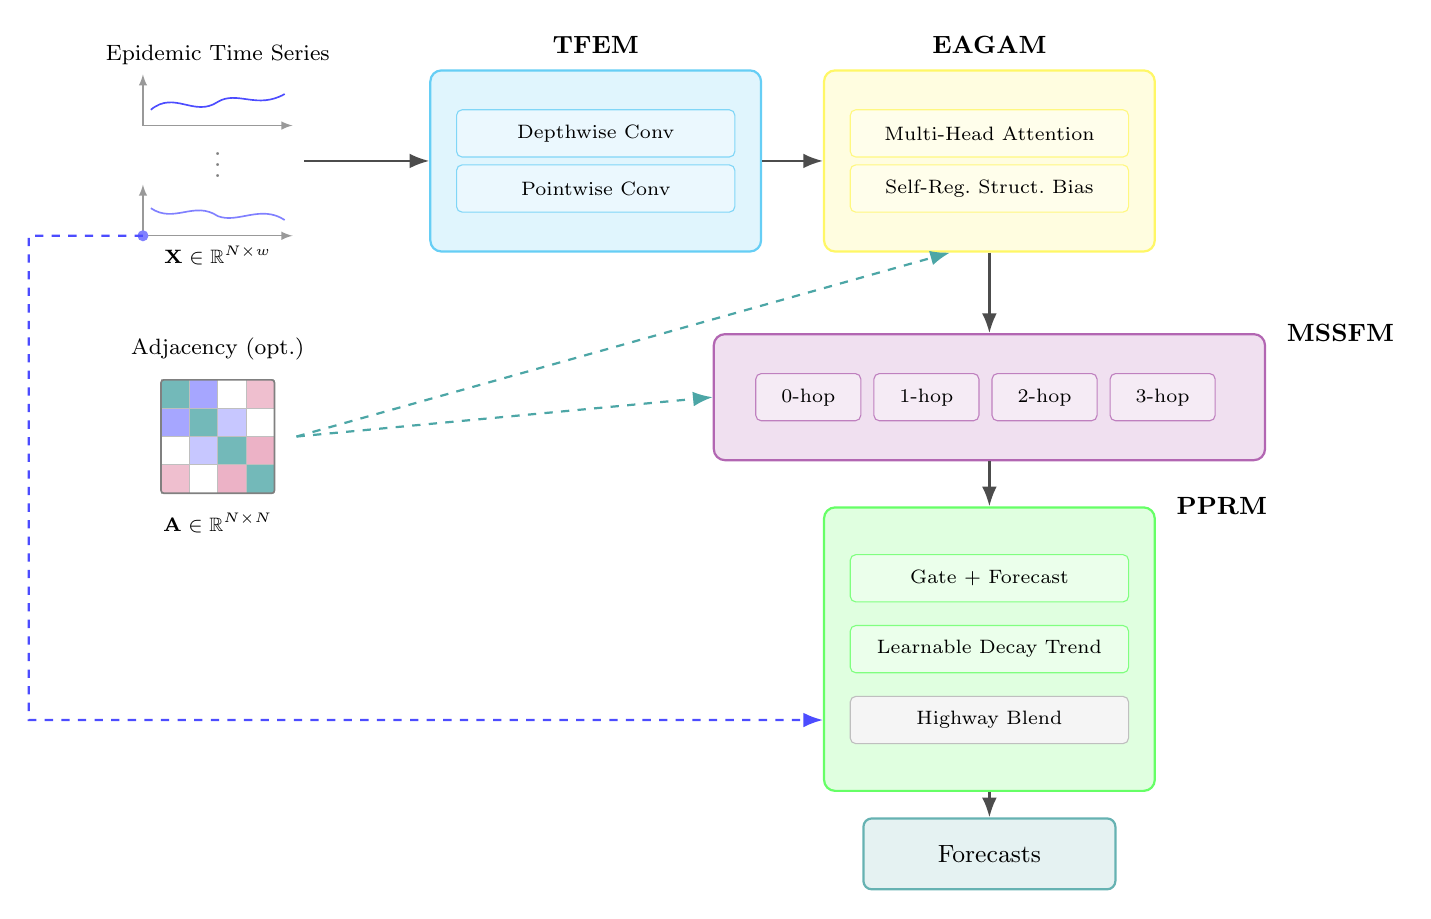
\begin{tikzpicture}[
        font=\small,
        >=latex,
        % --- Styles ---
        sblock/.style={
            rectangle, draw=#1!50, rounded corners=2pt,
            minimum height=0.6cm, text width=3.3cm,
            align=center, fill=#1!8, font=\scriptsize
        },
        iobox/.style={
            rectangle, draw=#1!60, thick, rounded corners=3pt,
            minimum height=0.9cm, minimum width=3.0cm,
            align=center, fill=#1!10, font=\small
        },
        modwrap/.style={
            rectangle, draw=#1!60, thick, rounded corners=4pt,
            align=center, fill=#1!12, inner sep=7pt
        },
        arr/.style={-{Latex[length=2.5mm]}, thick, black!70},
        darr/.style={-{Latex[length=2.5mm]}, dashed, thick, #1!70},
        lbl/.style={font=\small\bfseries, black}
    ]

    % ============================================================
    %  INPUT:  Two mini time-series plots with axes, dots between
    % ============================================================
    % --- Top time series (Region 1) ---
    \begin{scope}[shift={(-5.8, 0.7)}]
        \draw[->, black!40, thin] (-0.95, -0.25) -- (0.95, -0.25);
        \draw[->, black!40, thin] (-0.95, -0.25) -- (-0.95, 0.4);
        \draw[blue!70, semithick]
            (-0.85, -0.05)
            .. controls (-0.55, 0.2) and (-0.3, -0.15) .. (0.0, 0.05)
            .. controls (0.25, 0.2) and (0.5, -0.05) .. (0.85, 0.15);
    \end{scope}
    % --- Dots (regions 2 to N-1) ---
    \node[black!50, font=\normalsize] at (-5.8, 0.05) {$\vdots$};
    % --- Bottom time series (Region N) ---
    \begin{scope}[shift={(-5.8, -0.7)}]
        \draw[->, black!40, thin] (-0.95, -0.25) -- (0.95, -0.25);
        \draw[->, black!40, thin] (-0.95, -0.25) -- (-0.95, 0.4);
        \draw[blue!50, semithick]
            (-0.85, 0.1)
            .. controls (-0.55, -0.1) and (-0.3, 0.2) .. (0.0, 0.0)
            .. controls (0.25, -0.1) and (0.55, 0.15) .. (0.85, -0.05);
    \end{scope}
    \node[font=\footnotesize] at (-5.8, 1.35) {Epidemic Time Series};
    \node[font=\scriptsize] at (-5.8, -1.2) {$\mathbf{X}\in\mathbb{R}^{N\times w}$};
    \coordinate (IN) at (-4.7, 0);

    % ============================================================
    %  TFEM  (wider boxes so text fits)
    % ============================================================
    \node[modwrap=cyan, minimum height=2.3cm, minimum width=4.2cm] (tfem) at (-1.0, 0) {};
    \node[lbl, above=2pt of tfem] {TFEM};
    \node[sblock=cyan] (dw) at ([yshift=0.35cm]tfem.center) {Depthwise Conv};
    \node[sblock=cyan] (pw) at ([yshift=-0.35cm]tfem.center) {Pointwise Conv};

    % ============================================================
    %  EAGAM  (wider boxes so text fits)
    % ============================================================
    \node[modwrap=yellow, minimum height=2.3cm, minimum width=4.2cm] (eagam) at (4.0, 0) {};
    \node[lbl, above=2pt of eagam] {EAGAM};
    \node[sblock=yellow] (mha) at ([yshift=0.35cm]eagam.center) {Multi-Head Attention};
    \node[sblock=yellow] (srb) at ([yshift=-0.35cm]eagam.center) {Self-Reg.\ Struct.\ Bias};

    % Row 1 arrows
    \draw[arr] (IN) -- (tfem);
    \draw[arr] (tfem) -- (eagam);

    % ============================================================
    %  MSSFM  (label shifted right, away from arrow)
    % ============================================================
    \node[modwrap=violet, minimum height=1.6cm, minimum width=7.0cm]
        (mssfm) at (4.0, -3.0) {};
    \node[lbl, right=4pt] at (mssfm.north east) {MSSFM};
    \node[sblock=violet, text width=1.1cm] at ([xshift=-2.3cm]mssfm.center) {0-hop};
    \node[sblock=violet, text width=1.1cm] at ([xshift=-0.8cm]mssfm.center) {1-hop};
    \node[sblock=violet, text width=1.1cm] at ([xshift=0.7cm]mssfm.center)  {2-hop};
    \node[sblock=violet, text width=1.1cm] at ([xshift=2.2cm]mssfm.center)  {3-hop};

    \draw[arr] (eagam) -- (mssfm);

    % ============================================================
    %  PPRM  (includes Highway Blend; label shifted right)
    % ============================================================
    \node[modwrap=green, minimum height=3.6cm, minimum width=4.2cm]
        (pprm) at (4.0, -6.2) {};
    \node[lbl, right=4pt] at (pprm.north east) {PPRM};
    \node[sblock=green] (gf) at ([yshift=0.9cm]pprm.center)  {Gate + Forecast};
    \node[sblock=green] (dt) at (pprm.center)                 {Learnable Decay Trend};
    \node[sblock=gray]  (hw) at ([yshift=-0.9cm]pprm.center)  {Highway Blend};

    \draw[arr] (mssfm) -- (pprm);

    % ============================================================
    %  OUTPUT
    % ============================================================
    \node[iobox=teal, minimum width=3.2cm] (output) at (4.0, -8.8) {Forecasts};

    \draw[arr] (pprm) -- (output);

    % ============================================================
    %  ADJACENCY ICON  (heatmap-style matrix, multi-colour)
    % ============================================================
    \begin{scope}[shift={(-5.8, -3.5)}]
        \def\cs{0.36}          % cell size
        \def\ox{-0.72}         % grid left  = -4 half-cells
        \def\oy{-0.72}         % grid bottom
        %
        % --- Cell fills (symmetric matrix; diagonal = self-connection) ---
        % Row 0 (top row, i=0)
        \fill[teal!55]   (\ox,         \oy+3*\cs) rectangle +(\cs,\cs);  % (0,0) diag
        \fill[blue!35]   (\ox+\cs,     \oy+3*\cs) rectangle +(\cs,\cs);  % (0,1)
        \fill[white]     (\ox+2*\cs,   \oy+3*\cs) rectangle +(\cs,\cs);  % (0,2)
        \fill[purple!25] (\ox+3*\cs,   \oy+3*\cs) rectangle +(\cs,\cs);  % (0,3)
        % Row 1
        \fill[blue!35]   (\ox,         \oy+2*\cs) rectangle +(\cs,\cs);  % (1,0) sym
        \fill[teal!55]   (\ox+\cs,     \oy+2*\cs) rectangle +(\cs,\cs);  % (1,1) diag
        \fill[blue!22]   (\ox+2*\cs,   \oy+2*\cs) rectangle +(\cs,\cs);  % (1,2)
        \fill[white]     (\ox+3*\cs,   \oy+2*\cs) rectangle +(\cs,\cs);  % (1,3)
        % Row 2
        \fill[white]     (\ox,         \oy+\cs)   rectangle +(\cs,\cs);  % (2,0)
        \fill[blue!22]   (\ox+\cs,     \oy+\cs)   rectangle +(\cs,\cs);  % (2,1) sym
        \fill[teal!55]   (\ox+2*\cs,   \oy+\cs)   rectangle +(\cs,\cs);  % (2,2) diag
        \fill[purple!30] (\ox+3*\cs,   \oy+\cs)   rectangle +(\cs,\cs);  % (2,3)
        % Row 3 (bottom)
        \fill[purple!25] (\ox,         \oy)        rectangle +(\cs,\cs);  % (3,0) sym
        \fill[white]     (\ox+\cs,     \oy)        rectangle +(\cs,\cs);  % (3,1)
        \fill[purple!30] (\ox+2*\cs,   \oy)        rectangle +(\cs,\cs);  % (3,2) sym
        \fill[teal!55]   (\ox+3*\cs,   \oy)        rectangle +(\cs,\cs);  % (3,3) diag
        %
        % --- Grid lines ---
        \foreach \i in {0,...,4} {
            \draw[black!25, thin] (\ox+\i*\cs, \oy) -- (\ox+\i*\cs, \oy+4*\cs);
            \draw[black!25, thin] (\ox, \oy+\i*\cs) -- (\ox+4*\cs, \oy+\i*\cs);
        }
        % Outer border
        \draw[black!50, semithick, rounded corners=1pt]
            (\ox,\oy) rectangle (\ox+4*\cs, \oy+4*\cs);
        %
        \node[font=\footnotesize, above] at (0, 0.85) {Adjacency (opt.)};
        \node[font=\scriptsize, below] at (0, -0.85) {$\mathbf{A}\in\mathbb{R}^{N\times N}$};
    \end{scope}
    \coordinate (ADJ) at (-4.8, -3.5);

    % ============================================================
    %  ADJACENCY ARROWS  (clean diagonals, no crossing)
    % ============================================================
    \draw[darr=teal] (ADJ) -- ([xshift=-0.5cm]eagam.south);
    \draw[darr=teal] (ADJ) -- (mssfm.west);

    % ============================================================
    %  AUTOREGRESSIVE SKIP  (far-left route into Highway sub-block)
    % ============================================================
    \fill[blue!50] (-6.75, -0.95) circle (2pt);
    \draw[darr=blue]
        (-6.75, -0.95) -- (-8.2, -0.95) -- (-8.2, -7.1) -- ([yshift=-0.9cm]pprm.west);

    \end{tikzpicture}
    \caption{Overview of the MSAGAT-Net architecture. Epidemic time series for $N$ regions over a look-back window $w$ pass through TFEM, EAGAM, MSSFM, and PPRM before producing forecasts. PPRM incorporates the Highway Blend, which merges model predictions with an autoregressive baseline via a learnable gate~$\lambda$. Teal dashed lines indicate the optional adjacency matrix feeding into EAGAM (as a self-regulating soft prior) and MSSFM (for multi-hop aggregation); the blue dashed line marks the autoregressive skip connection.}
    \label{fig:msagat_net_architecture}
\end{figure*}

\subsection{Temporal Feature Extraction Module (TFEM)}

The first component of the MSAGAT-Net architecture is the Temporal Feature Extraction Module (TFEM), which transforms the raw time-series data into compact feature representations. Given input data $\mathbf{X} = [\mathbf{x}_{t-w+1}, \ldots, \mathbf{x}_t] \in \mathbb{R}^{N \times w}$ for $N$ regions over a look-back window of $w$ time steps, TFEM extracts temporal features through depthwise separable convolutions \cite{chollet2017xception} followed by low-rank projections, reducing parameter count and computational cost while maintaining expressive power \cite{li2023multi, yu2022traffic}.

\subsubsection{Depthwise Separable Convolutions}

For each region's historical window $\mathbf{x}^i_{[t-w+1:t]} \in \mathbb{R}^w$, we apply a depthwise convolution followed by a pointwise convolution. The depthwise convolution applies a separate filter per channel:

\begin{equation}
\mathbf{z}^i_{\text{depth}} = \text{Conv1D}_{\text{depth}}(\mathbf{x}^i; \boldsymbol{\Theta}_{\text{depth}})
\end{equation}

where $\mathbf{z}^i_{\text{depth}} \in \mathbb{R}^{w \times 1}$ represents the output after depthwise convolution, maintaining the temporal dimension whilst processing each input channel independently.

Following the depthwise convolution, a pointwise convolution (implemented as a 1×1 convolution) is applied to expand the single channel to multiple feature channels:

\begin{equation}
\mathbf{z}^i_{\text{point}} = \text{Conv1D}_{\text{point}}(\mathbf{z}^i_{\text{depth}}; \boldsymbol{\Theta}_{\text{point}})
\end{equation}

where $\mathbf{z}^i_{\text{point}} \in \mathbb{R}^{w \times d_{\text{feat}}}$ and $d_{\text{feat}} = 16$ is the number of output feature channels. Batch normalisation and ReLU activation are applied after each convolution:

\begin{equation}
\mathbf{z}^i_{\text{norm}} = \text{ReLU}(\text{BatchNorm}(\mathbf{z}^i_{\text{point}}))
\end{equation}

\subsubsection{Low-Rank Feature Projection}

After extracting features using depthwise separable convolutions, we apply a low-rank projection to further reduce dimensionality and capture the most salient features. This projection consists of two linear transformations with a bottleneck in between:

\begin{equation}
\mathbf{F}^i_{\text{low}} = \text{Linear}_{\text{low}}(\text{Flatten}(\mathbf{z}^i_{\text{norm}}))
\end{equation}

\begin{equation}
\mathbf{F}^i = \text{Linear}_{\text{high}}(\mathbf{F}^i_{\text{low}})
\end{equation}

where $\mathbf{F}^i_{\text{low}} \in \mathbb{R}^{d_{\text{bottle}}}$ is the bottleneck representation and $\mathbf{F}^i \in \mathbb{R}^{d_{\text{hidden}}}$ is the final feature vector for region $i$. The flattening operation converts $\mathbf{z}^i_{\text{norm}} \in \mathbb{R}^{w \times d_{\text{feat}}}$ into a vector of dimension $w \times d_{\text{feat}}$, which is then compressed through the bottleneck ($d_{\text{bottle}} \ll w \times d_{\text{feat}}$) before expansion to $d_{\text{hidden}}$. This low-rank bottleneck reduces the parameter count from $\mathcal{O}(w \cdot d_{\text{feat}} \cdot d_{\text{hidden}})$ to $\mathcal{O}(w \cdot d_{\text{feat}} \cdot d_{\text{bottle}} + d_{\text{bottle}} \cdot d_{\text{hidden}})$ per region, and acts as an information bottleneck that regularises the representations by forcing the model to retain only the most predictive temporal patterns.

After applying this projection to all regions, we obtain the feature matrix $\mathbf{F} \in \mathbb{R}^{N \times d_{\text{hidden}}}$ with layer normalisation and ReLU activation:

\begin{equation}
\mathbf{F} = \text{ReLU}(\text{LayerNorm}(\mathbf{F}))
\end{equation}

The TFEM pipeline is illustrated in Figure~\ref{fig:feature_extraction}.

All TFEM hyperparameters ($d_{\text{feat}}$, $d_{\text{bottle}}$, $d_{\text{hidden}}$, kernel size) are reported in Table~\ref{tab:hyperparameters}.

\begin{figure}
\centering
\resizebox{1.0\linewidth}{!}{%
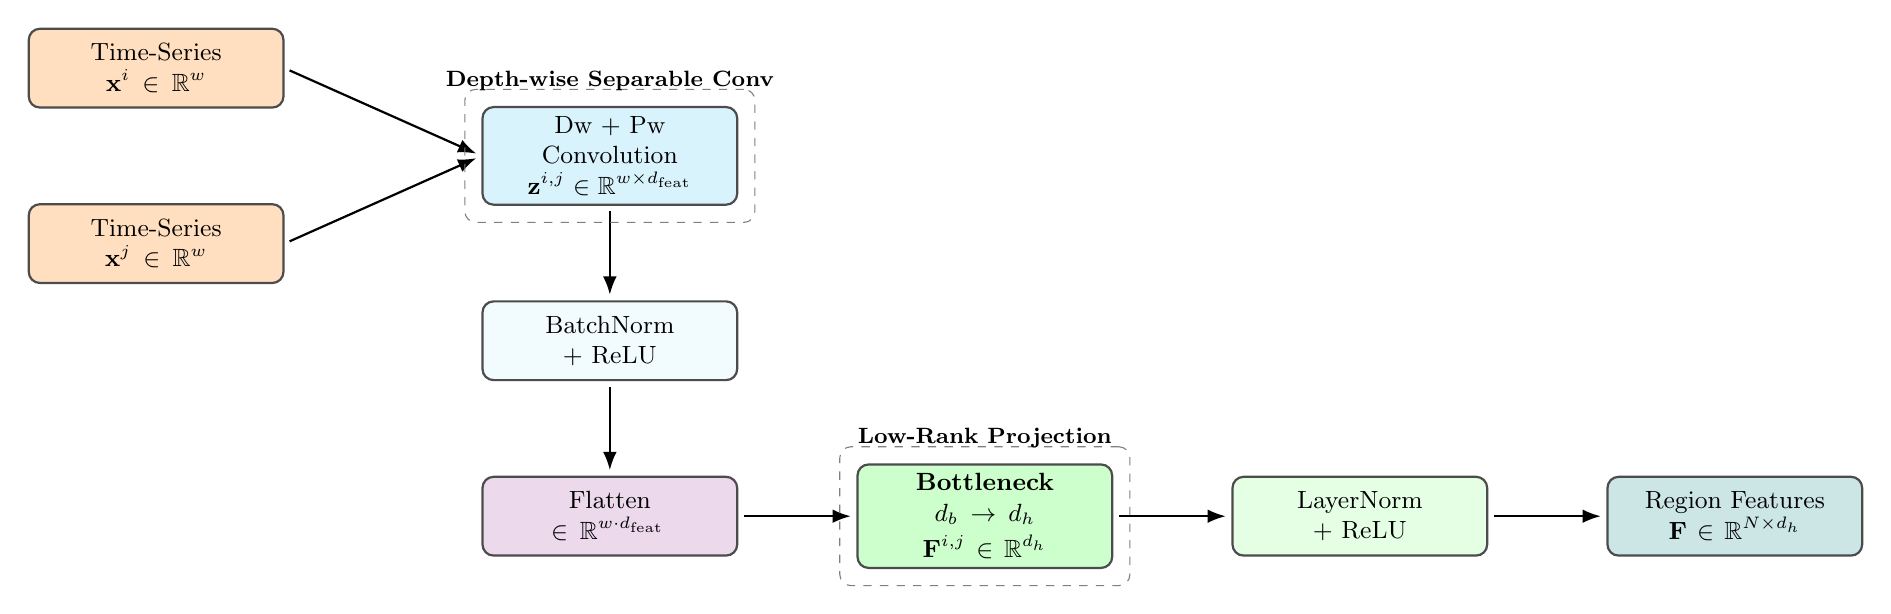
\begin{tikzpicture}[
    font=\small,
    >=Latex,
    block/.style={
        rectangle, draw=black!70, thick,
        rounded corners, align=center,
        minimum height=1cm,  % Increased height
        text width=3cm       % Increased width
    },
    arrow/.style={->, thick, shorten >=2pt, shorten <=2pt},
]
  %––– Inputs (split) –––––––––––––––––––––––––––––––––––––––
  \node (xi) [block, fill=orange!25] {Time‑Series\\$\mathbf{x}^i\!\in\!\mathbb{R}^{w}$};
  \node (xj) [block, fill=orange!25, below=1.2cm of xi] {Time‑Series\\$\mathbf{x}^j\!\in\!\mathbb{R}^{w}$};

  % Compute a point centred between xi and xj for tidy piping
  \path (xi.east) -- (xj.east) coordinate[midway] (midinput);

  %––– Pipeline nodes –––––––––––––––––––––––––––––––––––––––
  \node (sepconv) [block, fill=cyan!15,  right=2.5cm of midinput] {
      Dw + Pw\\Convolution\\
      $\mathbf{z}^{i,j}\!\in\!\mathbb{R}^{w\times d_{\text{feat}}}$};

  \node (bn)   [block, fill=cyan!5, below=1.2cm of sepconv] {BatchNorm\\+ ReLU};

  \node (flat) [block, fill=violet!15, below=1.2cm of bn] {Flatten\\$\!\in\!\mathbb{R}^{w\cdot d_{\text{feat}}}$};

  % Horizontal arrangement for the remaining nodes
  \node (proj) [block, fill=green!20, right=1.5cm of flat] {
      \textbf{Bottleneck}\\$d_b\!\to\! d_h$\\[2pt]
      $\mathbf{F}^{i,j}\!\in\!\mathbb{R}^{d_{h}}$};

  \node (ln) [block, fill=green!10, right=1.5cm of proj] {LayerNorm\\+ ReLU};

  \node (output) [block, fill=teal!20, right=1.5cm of ln] {Region Features\\$\mathbf{F}\!\in\!\mathbb{R}^{N\times d_{h}}$};

  %––– Arrows –––––––––––––––––––––––––––––––––––––––––––––––
  \draw[arrow] (xi.east) -- (sepconv.west);
  \draw[arrow] (xj.east) -- (sepconv.west);
  \draw[arrow] (sepconv.south) -- ++(0,-0.6) -- (bn.north);
  \draw[arrow] (bn.south) -- ++(0,-0.6) -- (flat.north);
  \draw[arrow] (flat.east) -- (proj.west);
  \draw[arrow] (proj.east) -- (ln.west);
  \draw[arrow] (ln.east) -- (output.west);

  %––– Grouping boxes –––––––––––––––––––––––––––––––––––––––
  % \begin{scope}[on background layer] % Removed for IEEEtran compatibility
    \node[draw=black!50, dashed, rounded corners, inner sep=6pt,
          fit=(sepconv)] {};
    \node at (sepconv.north) [above=2pt, font=\footnotesize\bfseries] {Depth‑wise Separable Conv};

    \node[draw=black!50, dashed, rounded corners, inner sep=6pt,
          fit=(proj)] {};
    \node at (proj.north) [above=2pt, font=\footnotesize\bfseries] {Low‑Rank Projection};
  % \end{scope} % Removed for IEEEtran compatibility
\end{tikzpicture}%
}
\caption{Feature‑extraction pipeline. Independent regional time‑series $\mathbf{x}^i$ and $\mathbf{x}^j$ are processed in parallel by depth‑wise and point‑wise convolutions, normalised, flattened, passed through a bottleneck projection ($d_{\text{bottle}}\!\to\! d_{\text{hidden}}$), and normalised again to yield region‑level feature vectors $\mathbf F$.}
\label{fig:feature_extraction}
\end{figure}

\subsection{Efficient Adaptive Graph Attention with Low-Rank Decomposition}

The second core component of our MSAGAT-Net architecture is EAGAM. Traditional approaches to spatial modelling often rely on fixed adjacency matrices based on geographical proximity or administrative boundaries, which do not capture the evolving nature of epidemic spread influenced by factors such as population mobility, healthcare referral patterns, and socioeconomic connections. Based on the principles of graph attention networks \cite{velickovic2017graph}, our EAGAM adaptively learns the relationships between regions based on their feature representations, rather than being constrained by a predefined graph structure. This adaptive approach allows the model to discover and leverage spatial dependencies that may not be immediately apparent from geographical proximity alone, and to adjust these dependencies as the epidemic evolves.

Standard graph attention mechanisms incur $\mathcal{O}(N^2 \cdot d)$ complexity and offer no mechanism to control how much structural prior influences the learned attention. Low-rank decomposition has been shown to reduce this cost effectively \cite{puny2020global, kong2023low, yang2023self}, motivating the design of EAGAM.

EAGAM employs multi-head scaled dot-product attention with low-rank bottleneck projections for query, key, and value representations. Its key innovation is the integration of two complementary structural biases directly into the attention scores \emph{before} softmax normalisation: (i) a learnable low-rank graph bias $\mathbf{B} = \mathbf{UV}$ that captures persistent spatial relationships from data, and (ii) an optional additive adjacency prior with learnable scale whose influence self-regulates based on graph density (detailed in Section~\ref{sec:adj_prior}). The module comprises five components described below.


\subsubsection{Bottleneck Projection}

Given the feature matrix $\mathbf{F} \in \mathbb{R}^{N \times d_{\text{hidden}}}$ from TFEM, where $N$ is the number of regions and $d_{\text{hidden}}$ is the hidden dimension, we first project these features into query, key, and value representations through an efficient bottleneck projection:

\begin{equation}
\mathbf{Q}_{\text{low}}, \mathbf{K}_{\text{low}}, \mathbf{V}_{\text{low}} = \text{Split}(\text{Linear}_{\text{low}}(\mathbf{F}), 3)
\end{equation}

where $\text{Linear}_{\text{low}}: \mathbb{R}^{d_{\text{hidden}}} \rightarrow \mathbb{R}^{3 \times d_{\text{bottle}}}$ projects the features into a lower-dimensional space and $\text{Split}$ divides the output into three separate tensors of dimension $\mathbb{R}^{N \times d_{\text{bottle}}}$.

These low-dimensional projections are then expanded back to the full hidden dimension:

\begin{equation}
\mathbf{Q}, \mathbf{K}, \mathbf{V} = \text{Split}(\text{Linear}_{\text{high}}([\mathbf{Q}_{\text{low}}; \mathbf{K}_{\text{low}}; \mathbf{V}_{\text{low}}]), 3)
\end{equation}

where $\text{Linear}_{\text{high}}: \mathbb{R}^{3 \times d_{\text{bottle}}} \rightarrow \mathbb{R}^{3 \times d_{\text{hidden}}}$ and each of $\mathbf{Q}, \mathbf{K}, \mathbf{V} \in \mathbb{R}^{N \times d_{\text{hidden}}}$.

This bottleneck projection significantly reduces the parameter count from $\mathcal{O}(3 \times d_{\text{hidden}}^2)$ to $\mathcal{O}(3 \times d_{\text{hidden}} \times d_{\text{bottle}})$, where $d_{\text{bottle}} \ll d_{\text{hidden}}$.

\subsubsection{Multi-Head Attention Mechanism}

To enhance the model's capacity to capture different types of inter-regional relationships, we implement a multi-head attention mechanism where the hidden representations are split into $h$ heads, each with dimension $d_{\text{head}} = d_{\text{hidden}} / h$:

\begin{equation}
\mathbf{Q}^{(i)}, \mathbf{K}^{(i)}, \mathbf{V}^{(i)} \in \mathbb{R}^{N \times d_{\text{head}}}, \quad i \in \{1, 2, \ldots, h\}
\end{equation}

For efficient computation, we reshape these tensors to explicitly represent the multiple heads:

\begin{equation}
\mathbf{Q}_h = \text{Reshape}(\mathbf{Q}, [N, h, d_{\text{head}}])
\end{equation}
\begin{equation}
\mathbf{K}_h = \text{Reshape}(\mathbf{K}, [N, h, d_{\text{head}}])
\end{equation}
\begin{equation}
\mathbf{V}_h = \text{Reshape}(\mathbf{V}, [N, h, d_{\text{head}}])
\end{equation}

We then transpose the first two dimensions to facilitate batch-wise processing across attention heads:

\begin{align}
\mathbf{Q}_h &= \text{Transpose}(\mathbf{Q}_h, 0, 1) \\
\mathbf{K}_h &= \text{Transpose}(\mathbf{K}_h, 0, 1) \\
\mathbf{V}_h &= \text{Transpose}(\mathbf{V}_h, 0, 1)
\end{align}

resulting in tensors of shape $[h, N, d_{\text{head}}]$.

Within each attention head, we compute standard scaled dot-product attention scores:

\begin{equation}
\mathbf{S}_h = \frac{\mathbf{Q}_h \mathbf{K}_h^T}{\sqrt{d_{\text{head}}}}
\end{equation}

where $\mathbf{S}_h \in \mathbb{R}^{h \times N \times N}$. The two structural biases---a learnable graph bias $\mathbf{B}$ (Section~\ref{sec:graph_bias}) and an optional adjacency prior (Section~\ref{sec:adj_prior})---are added before softmax normalisation:

\begin{equation}
\mathbf{A}_h = \text{softmax}(\mathbf{S}_h + \mathbf{B} + \alpha \cdot \tilde{\mathbf{A}})
\end{equation}

where $\mathbf{B} = \mathbf{UV}$ is the learnable graph bias, $\tilde{\mathbf{A}}$ is the row-normalised adjacency prior (when available), and $\alpha = \text{softplus}(\alpha_0)$ is a learnable positive scale parameter. The self-regulating properties of this additive formulation are analysed in Section~\ref{sec:adj_prior}.

The final attention output for each head is then computed as:

\begin{equation}
\mathbf{O}_h = \mathbf{A}_h \mathbf{V}_h
\end{equation}

where $\mathbf{O}_h \in \mathbb{R}^{h \times N \times d_{\text{head}}}$ represents the attended features across all heads.

\subsubsection{Learnable Graph Structure Bias}
\label{sec:graph_bias}

An important feature of our EAGAM is the incorporation of a learnable graph structure bias that is added directly to the attention scores before softmax normalisation. Unlike traditional graph attention networks that rely solely on node features for computing attention, we include a learnable bias term that captures persistent structural relationships between regions that may not be evident from the node features alone.

This bias is implemented as a low-rank decomposition for parameter efficiency:

\begin{equation}
\mathbf{B} = \mathbf{U} \mathbf{V}
\end{equation}

where $\mathbf{U} \in \mathbb{R}^{h \times N \times d_{\text{bias}}}$ and $\mathbf{V} \in \mathbb{R}^{h \times d_{\text{bias}} \times N}$ are learnable parameters initialised with Xavier uniform \cite{glorot2010understanding}, and $d_{\text{bias}} \ll N$ is the bottleneck dimension. The resulting bias $\mathbf{B} \in \mathbb{R}^{h \times N \times N}$ is added directly to the content-based attention scores before softmax, allowing it to reinforce or suppress specific region-to-region attention patterns as a first-class component of the spatial reasoning mechanism.

\subsubsection{Self-Regulating Additive Adjacency Prior}
\label{sec:adj_prior}

Unlike state-of-the-art baselines that \emph{require} predefined adjacency matrices, MSAGAT-Net learns spatial relationships entirely from data. However, when prior knowledge about regional connectivity is available (e.g., geographical proximity or mobility patterns), it can be optionally incorporated to accelerate learning and improve performance through an additive prior mechanism.

Given an adjacency matrix $\mathbf{A}$, we first compute a row-normalised prior:

\begin{equation}
\tilde{\mathbf{A}} = \mathbf{D}_{\text{row}}^{-1}\mathbf{A}
\end{equation}

where $\mathbf{D}_{\text{row}} = \text{diag}(\mathbf{A}\mathbf{1})$ is the row-sum diagonal matrix. This prior is then added to the attention scores with a learnable positive scale:

\begin{equation}
\mathbf{S}_h' = \mathbf{S}_h + \mathbf{B} + \alpha \cdot \tilde{\mathbf{A}}
\end{equation}

where $\alpha = \text{softplus}(\alpha_0)$ ensures positivity, and $\alpha_0$ is a learnable scalar parameter initialised to $1.0$ (yielding $\alpha \approx 1.31$ initially, providing a moderate structural nudge).

The key insight behind this additive formulation is its \emph{self-regulating} behaviour across different graph topologies. Because the softmax function is shift-invariant---$\text{softmax}(\mathbf{x} + c\mathbf{1}) = \text{softmax}(\mathbf{x})$ for any constant vector $c\mathbf{1}$---the prior's effect naturally adapts to graph density:

\begin{itemize}
    \item \textbf{Dense graphs:} When the adjacency matrix is dense, the row-normalised prior $\tilde{\mathbf{A}}$ approaches a uniform distribution across all columns. Adding a near-constant vector to each row of attention scores before softmax has negligible effect on the resulting attention distribution. The model thus relies primarily on content-based attention and the learned graph bias.
    \item \textbf{Sparse graphs:} When the adjacency matrix is sparse, $\tilde{\mathbf{A}}$ has peaked entries for connected nodes and zeros elsewhere. The additive prior meaningfully shifts attention towards geographically relevant neighbours, providing structural guidance where it is most needed.
\end{itemize}

This self-regulating property eliminates the need for graph-size-dependent thresholds or conditional gating mechanisms, which we found to be fragile in practice. When no adjacency is provided, the model operates using only content-based attention and the learned graph bias; when adjacency is available, the scale $\alpha$ is learned during training, and the prior is pre-computed and stored as a constant buffer with negligible overhead. This distinguishes MSAGAT-Net from baselines such as EpiGNN \cite{xie2022epignn}, Cola-GNN \cite{deng2020cola}, and DCRNN \cite{li2018diffusion}, which mandate adjacency matrices as required input.

\subsubsection{Attention Regularisation}

To promote sparse and interpretable spatial relationships, we apply L1 regularisation to the attention weight matrix after softmax normalisation:

\begin{equation}
\mathcal{L}_{\text{attn}} = \lambda \|\mathbf{A}_h\|_1
\end{equation}

where $\mathbf{A}_h$ denotes the attention weights (the softmax output used for value aggregation) and $\lambda$ is a learnable regularisation weight. By penalising the L1 norm of the attention distribution rather than the structural bias alone, this regularisation directly encourages each node to attend to a sparse subset of other nodes, producing interpretable spatial dependency patterns. The value of $\lambda$ is initialised to $10^{-5}$ and adapted during training through gradient descent in log-domain (ensuring positivity), allowing the model to automatically balance forecast accuracy with attention sparsity.

After computing the attended values for each head, we combine them and project back to the original feature dimension:

\begin{equation}
\mathbf{O} = \text{Reshape}(\text{Transpose}(\mathbf{O}_h, 0, 1), [N, d_{\text{hidden}}])
\end{equation}

Similarly to the input projection, we employ a low-rank output projection for efficiency:

\begin{equation}
\mathbf{O}_{\text{low}} = \text{Linear}_{\text{out\_low}}(\mathbf{O})
\end{equation}

\begin{equation}
\mathbf{O}_{\text{final}} = \text{Linear}_{\text{out\_high}}(\mathbf{O}_{\text{low}})
\end{equation}

where $\mathbf{O}_{\text{low}} \in \mathbb{R}^{N \times d_{\text{bottle}}}$ and $\mathbf{O}_{\text{final}} \in \mathbb{R}^{N \times d_{\text{hidden}}}$.

The output of EAGAM, $\mathbf{O}_{\text{final}}$, represents the features of the region after incorporating spatial dependencies. This output, along with the attention regularisation loss $\mathcal{L}_{\text{attn}}$, is passed to the subsequent MSSFM for further processing.

All EAGAM hyperparameters (attention heads, bottleneck dimension, regularisation weight, adjacency prior scale) are reported in Table~\ref{tab:hyperparameters}. Figure~\ref{fig:eagam_module} presents the data flow through the EAGAM module.

\begin{figure}
\centering
\resizebox{0.85\linewidth}{!}{%
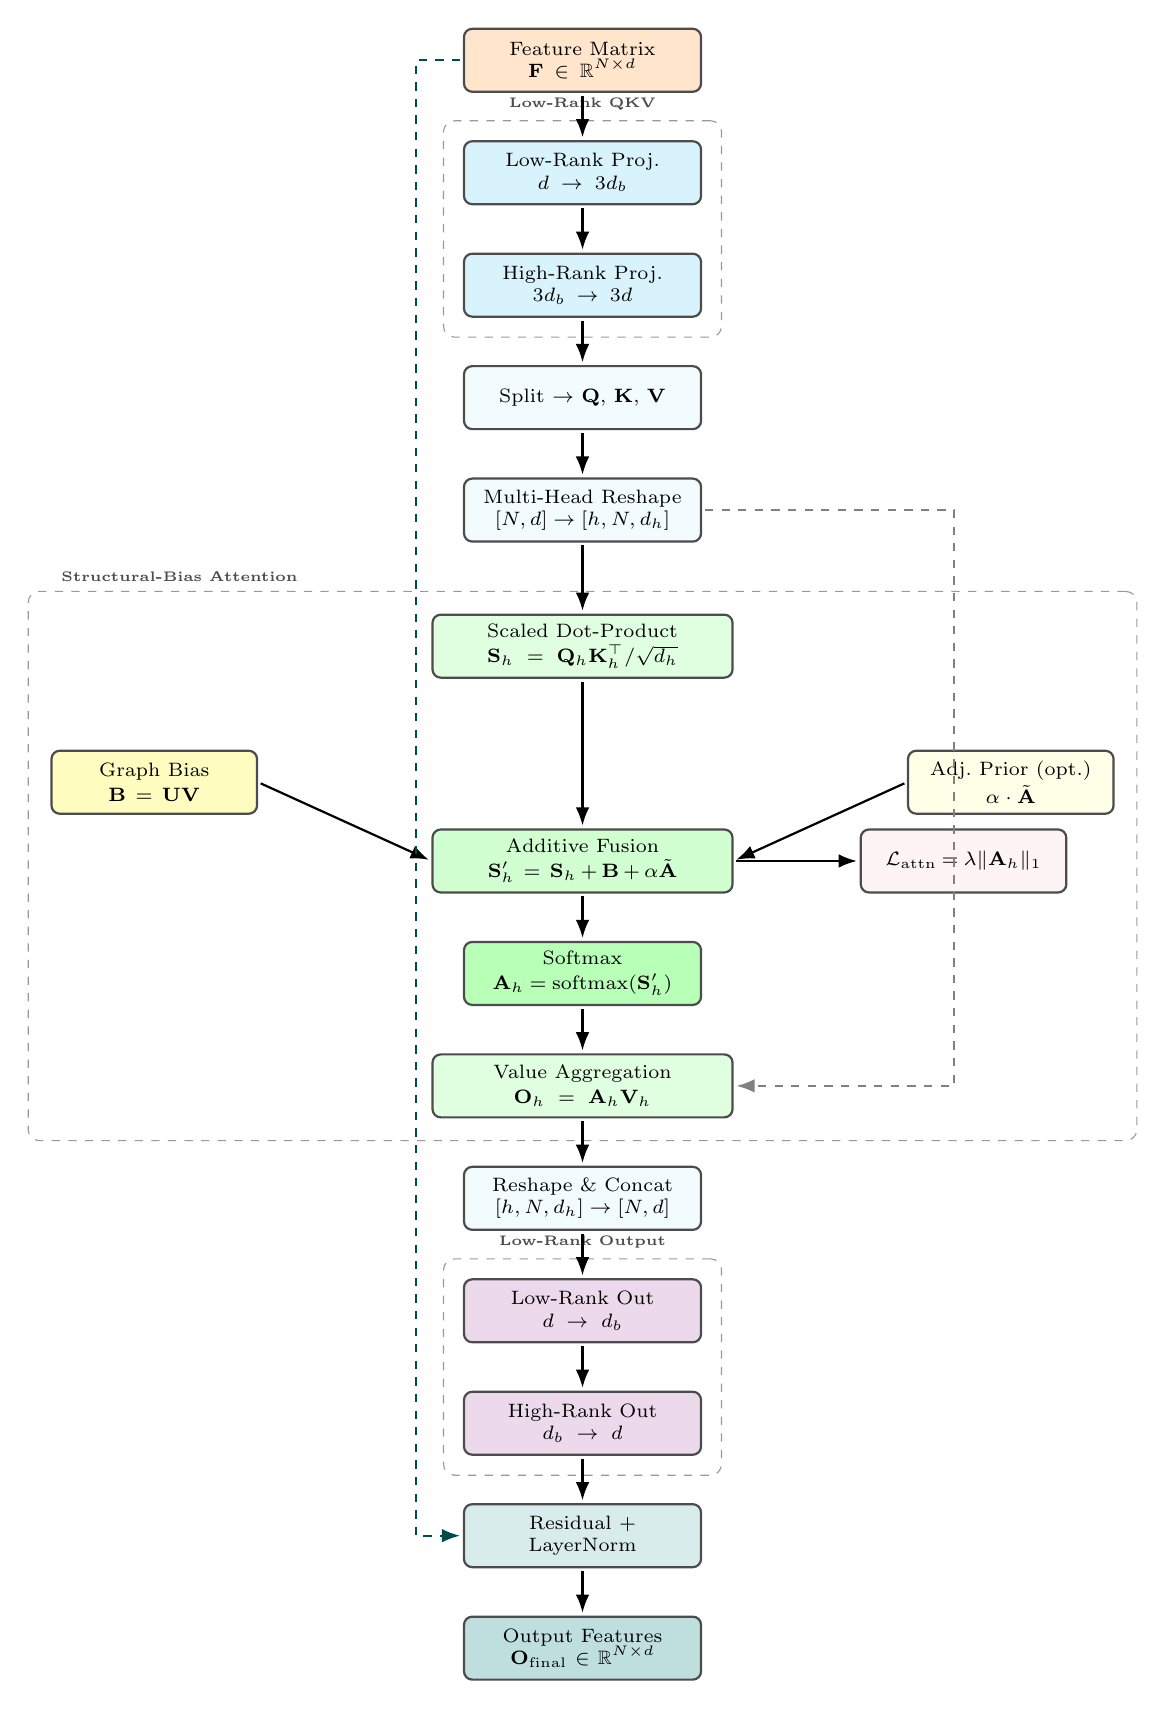
\begin{tikzpicture}[
    font=\scriptsize,
    >=Latex,
    node distance = 0.6cm and 1.4cm,
    % --- node styles ---
    block/.style = {rectangle, draw=black!70, thick,
                    rounded corners=3pt, align=center,
                    minimum height=0.8cm,
                    text width=2.8cm,
                    inner sep=3pt},
    wblock/.style = {block, text width=3.6cm},
    sideblock/.style = {block, text width=2.4cm},
    arrow/.style  = {->, thick, shorten >=1pt, shorten <=1pt},
    darrow/.style = {->, thick, dashed, shorten >=1pt, shorten <=1pt},
    grouplbl/.style = {font=\tiny\bfseries, text=black!70},
]

%============ INPUT ============
\node (input) [block, fill=orange!20]
  {Feature Matrix\\$\mathbf{F}\!\in\!\mathbb{R}^{N\times d}$};

%============ LOW-RANK QKV PROJECTION ============
\node (qkv_low) [block, fill=cyan!15, below=of input]
  {Low-Rank Proj.\\$d \!\to\! 3d_b$};

\node (qkv_high) [block, fill=cyan!15, below=of qkv_low]
  {High-Rank Proj.\\$3d_b \!\to\! 3d$};

\node (split) [block, fill=cyan!5, below=of qkv_high]
  {Split $\to$ $\mathbf{Q}$, $\mathbf{K}$, $\mathbf{V}$};

\node (reshape) [block, fill=cyan!5, below=of split]
  {Multi-Head Reshape\\$[N,d]\!\to\![h,N,d_h]$};

%============ CONTENT ATTENTION ============
\node (dotprod) [wblock, fill=green!12, below=0.9cm of reshape]
  {Scaled Dot-Product\\[1pt]
   $\mathbf{S}_h = \mathbf{Q}_h\mathbf{K}_h^\top / \sqrt{d_h}$};

%============ STRUCTURAL BIASES (side branches) ============
\node (gbias) [sideblock, fill=yellow!25, below left=0.9cm and 2.2cm of dotprod]
  {Graph Bias\\[1pt]$\mathbf{B}\!=\!\mathbf{U}\mathbf{V}$};

\node (adjpr) [sideblock, fill=yellow!10, below right=0.9cm and 2.2cm of dotprod]
  {Adj.\ Prior (opt.)\\[1pt]$\alpha\!\cdot\!\tilde{\mathbf{A}}$};

%============ ADDITIVE FUSION ============
\node (addfuse) [wblock, fill=green!18, below=1.9cm of dotprod]
  {Additive Fusion\\[1pt]
   $\mathbf{S}_h'\!=\!\mathbf{S}_h\!+\!\mathbf{B}\!+\!\alpha\tilde{\mathbf{A}}$};

%============ SOFTMAX ============
\node (softmax) [block, fill=green!28, below=of addfuse]
  {Softmax\\[1pt]
   $\mathbf{A}_h\!=\!\mathrm{softmax}(\mathbf{S}_h')$};

%============ VALUE AGGREGATION ============
\node (valagg) [wblock, fill=green!12, below=of softmax]
  {Value Aggregation\\[1pt]
   $\mathbf{O}_h\!=\!\mathbf{A}_h\mathbf{V}_h$};

%============ REGULARISATION (side) ============
\node (reg) [sideblock, fill=pink!18, right=1.6cm of addfuse]
  {$\mathcal{L}_{\mathrm{attn}}\!=\!\lambda\|\mathbf{A}_h\|_1$};

%============ OUTPUT PATH ============
\node (reshapeout) [block, fill=cyan!5, below=of valagg]
  {Reshape \& Concat\\$[h,N,d_h]\!\to\![N,d]$};

\node (outlow) [block, fill=violet!15, below=of reshapeout]
  {Low-Rank Out\\$d\!\to\! d_b$};

\node (outhigh) [block, fill=violet!15, below=of outlow]
  {High-Rank Out\\$d_b\!\to\! d$};

\node (resid) [block, fill=teal!15, below=of outhigh]
  {Residual + LayerNorm};

\node (output) [block, fill=teal!25, below=of resid]
  {Output Features\\$\mathbf{O}_{\mathrm{final}}\!\in\!\mathbb{R}^{N\times d}$};

%============ MAIN-FLOW ARROWS ============
\foreach \a/\b in {
  input/qkv_low, qkv_low/qkv_high, qkv_high/split, split/reshape,
  reshape/dotprod, dotprod/addfuse,
  addfuse/softmax, softmax/valagg,
  valagg/reshapeout, reshapeout/outlow, outlow/outhigh, outhigh/resid, resid/output}
  \draw[arrow] (\a) -- (\b);

% Structural-bias arrows into additive fusion
\draw[arrow] (gbias.east)  -- (addfuse.west);
\draw[arrow] (adjpr.west)  -- (addfuse.east);

% Reg arrow
\draw[arrow] (addfuse) -- (reg);

% V path bypass (dashed): from reshape directly to value aggregation
\draw[darrow, gray] (reshape.east) -- ++(3.2,0) |- (valagg.east);

% Residual skip connection from input to residual+LN node
\draw[darrow, teal!60!black]
  (input.west) -- ++(-0.6,0) |- (resid.west);

%============ GROUP BOXES (background) ============
\begin{scope}[on background layer]
  % Low-Rank QKV group
  \node [draw=black!40, dashed, rounded corners=4pt, inner sep=7pt,
         fit=(qkv_low)(qkv_high), label={[grouplbl]above:Low-Rank QKV}] {};

  % Structural-Bias Attention group
  \node [draw=black!40, dashed, rounded corners=4pt, inner sep=8pt,
         fit=(dotprod)(gbias)(adjpr)(addfuse)(softmax)(valagg),
         label={[grouplbl]above left:Structural-Bias Attention}] {};

  % Low-Rank Output group
  \node [draw=black!40, dashed, rounded corners=4pt, inner sep=7pt,
         fit=(outlow)(outhigh), label={[grouplbl]above:Low-Rank Output}] {};
\end{scope}

\end{tikzpicture}}%
\caption{Data flow in the EAGAM module. Input features $\mathbf{F}$ are projected through a low-rank bottleneck into Q, K, V representations. Scaled dot-product scores are augmented with a learnable graph bias $\mathbf{B}=\mathbf{UV}$ and an optional adjacency prior $\alpha\cdot\tilde{\mathbf{A}}$ before softmax. Attended values pass through a low-rank output stage with residual connection. $\mathcal{L}_{\mathrm{attn}}$: L1 sparsity loss on attention weights.}
\label{fig:eagam_module}
\end{figure}

\subsection{Multi-Scale Spatial Feature Module}

The third major component of the proposed MSAGAT-Net architecture is the Multi-Scale Spatial Feature Module (MSSFM), which refines spatial dependencies using multi-hop graph convolutions. Epidemic propagation involves interactions that extend beyond immediate neighbours, but excessive diffusion can oversmooth small graphs. MSSFM addresses this by aggregating information across multiple hop distances while adaptively limiting the maximum hop depth based on graph size and fusing scales with locality-biased weights.

\subsubsection{Multi-Hop Graph Convolutions}

Let $\mathbf{G} \in \mathbb{R}^{B \times N \times d_{\text{hidden}}}$ denote the spatial features output by EAGAM. Given an adjacency matrix $\mathbf{A}$, we construct a row-normalised matrix with self-loops:

\begin{equation}
\mathbf{\hat{A}} = \mathbf{D}^{-1}(\mathbf{A} + \mathbf{I}),
\end{equation}

where $\mathbf{D}$ is the degree matrix of $(\mathbf{A} + \mathbf{I})$. For each hop $k \in \{0, 1, \ldots, S-1\}$, MSSFM computes a k-hop aggregation:

\begin{equation}
\mathbf{H}^{(k)} = \mathbf{\hat{A}}^{k}\mathbf{G}\mathbf{W}^{(k)},
\end{equation}

with $\mathbf{W}^{(k)}$ implemented as a linear transform followed by LayerNorm and ReLU. The $k=0$ scale uses the identity matrix to preserve self-features. When no adjacency is provided, MSSFM defaults to identity aggregation across all scales.

\subsubsection{Adaptive Hop Depth and Locality-Biased Fusion}

To reduce oversmoothing on small graphs, the number of scales is set adaptively as
\begin{equation}
S = \min(S_{\max}, \max(2, \lfloor N/5 \rfloor)),
\end{equation}
ensuring that small graphs use fewer hops while larger graphs retain broader context. We fuse the multi-hop features with learnable weights initialised to favour locality:

\begin{equation}
\boldsymbol{\alpha} = \text{softmax}(\mathbf{w}), \quad
\mathbf{H}_{\text{fused}} = \sum_{k=0}^{S-1} \alpha_k \mathbf{H}^{(k)}.
\end{equation}

\subsubsection{Bottleneck Projection and Residual Connection}

The fused features are passed through a low-rank bottleneck projection and residual connection to stabilise training:

\begin{equation}
\mathbf{H}_{\text{proj}} = \text{Linear}_{\text{high}}(\text{Linear}_{\text{low}}(\mathbf{H}_{\text{fused}})),
\end{equation}
\begin{equation}
\mathbf{H}_{\text{final}} = \text{LayerNorm}(\mathbf{H}_{\text{proj}} + \mathbf{G}).
\end{equation}

This design preserves the hidden dimension while enabling adaptive spatial refinement across multiple hop distances. Figure~\ref{fig:mssfm_module} illustrates the data flow through the MSSFM module.

\begin{figure}[!ht]
\centering
\resizebox{0.92\linewidth}{!}{%
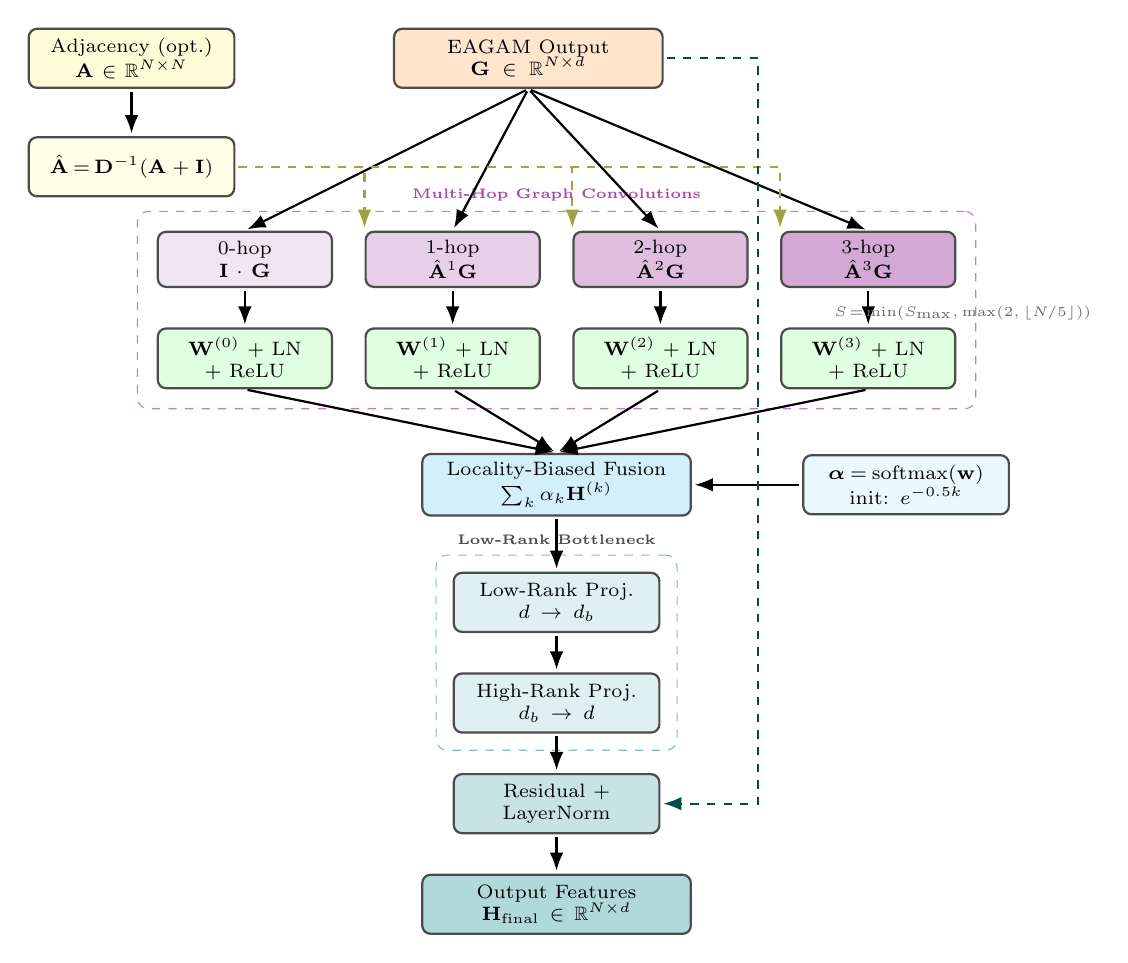
\begin{tikzpicture}[
    font=\scriptsize,
    >=Latex,
    node distance = 0.55cm and 1.0cm,
    % --- node styles ---
    block/.style = {rectangle, draw=black!70, thick,
                    rounded corners=3pt, align=center,
                    minimum height=0.75cm,
                    text width=2.4cm,
                    inner sep=3pt},
    wblock/.style = {block, text width=3.2cm},
    hopblock/.style = {block, minimum height=0.7cm, text width=2.0cm},
    arrow/.style  = {->, thick, shorten >=1pt, shorten <=1pt},
    darrow/.style = {->, thick, dashed, shorten >=1pt, shorten <=1pt},
    grouplbl/.style = {font=\tiny\bfseries, text=black!70},
]

%============ INPUT ============
\node (input) [wblock, fill=orange!20]
  {EAGAM Output\\$\mathbf{G}\!\in\!\mathbb{R}^{N\times d}$};

%============ ADJACENCY ============
\node (adj) [block, fill=yellow!15, left=2.0cm of input]
  {Adjacency (opt.)\\$\mathbf{A}\!\in\!\mathbb{R}^{N\times N}$};

\node (adjhat) [block, fill=yellow!10, below=0.6cm of adj]
  {$\hat{\mathbf{A}}\!=\!\mathbf{D}^{-1}(\mathbf{A}+\mathbf{I})$};

\draw[arrow] (adj) -- (adjhat);

%============ PARALLEL HOP BRANCHES ============
% Position them below the input, spaced horizontally
\node (hop0) [hopblock, fill=violet!10, below=1.8cm of input, xshift=-3.6cm]
  {0-hop\\$\mathbf{I}\cdot\mathbf{G}$};
\node (hop1) [hopblock, fill=violet!18, right=0.4cm of hop0]
  {1-hop\\$\hat{\mathbf{A}}^1\mathbf{G}$};
\node (hop2) [hopblock, fill=violet!26, right=0.4cm of hop1]
  {2-hop\\$\hat{\mathbf{A}}^2\mathbf{G}$};
\node (hop3) [hopblock, fill=violet!34, right=0.4cm of hop2]
  {3-hop\\$\hat{\mathbf{A}}^3\mathbf{G}$};

% Input feeds all hops
\foreach \h in {hop0,hop1,hop2,hop3}
  \draw[arrow] (input.south) -- (\h.north);

% Adjacency powers feed hops 1--3
\draw[darrow, yellow!60!black] (adjhat.east) -| (hop1.north west);
\draw[darrow, yellow!60!black] (adjhat.east) -| (hop2.north west);
\draw[darrow, yellow!60!black] (adjhat.east) -| (hop3.north west);

%============ PER-HOP TRANSFORMS ============
\node (w0) [hopblock, fill=green!12, below=0.5cm of hop0]
  {$\mathbf{W}^{(0)}$ + LN + ReLU};
\node (w1) [hopblock, fill=green!12, below=0.5cm of hop1]
  {$\mathbf{W}^{(1)}$ + LN + ReLU};
\node (w2) [hopblock, fill=green!12, below=0.5cm of hop2]
  {$\mathbf{W}^{(2)}$ + LN + ReLU};
\node (w3) [hopblock, fill=green!12, below=0.5cm of hop3]
  {$\mathbf{W}^{(3)}$ + LN + ReLU};

\foreach \h/\w in {hop0/w0, hop1/w1, hop2/w2, hop3/w3}
  \draw[arrow] (\h) -- (\w);

%============ ADAPTIVE FUSION ============
\node (fusion) [wblock, fill=cyan!18, below=1.2cm of $(w1)!0.5!(w2)$]
  {Locality-Biased Fusion\\$\sum_k \alpha_k \mathbf{H}^{(k)}$};

\foreach \w in {w0,w1,w2,w3}
  \draw[arrow] (\w.south) -- (fusion.north);

% Alpha weights annotation
\node (alpha) [block, fill=cyan!8, right=1.4cm of fusion]
  {$\boldsymbol{\alpha}\!=\!\mathrm{softmax}(\mathbf{w})$\\init: $e^{-0.5k}$};
\draw[arrow] (alpha) -- (fusion);

%============ BOTTLENECK + RESIDUAL ============
\node (bnlow) [block, fill=teal!12, below=0.7cm of fusion]
  {Low-Rank Proj.\\$d\!\to\! d_b$};

\node (bnhigh) [block, fill=teal!12, below=0.5cm of bnlow]
  {High-Rank Proj.\\$d_b\!\to\! d$};

\node (resid) [block, fill=teal!22, below=0.5cm of bnhigh]
  {Residual + LayerNorm};

\node (output) [wblock, fill=teal!30, below=0.5cm of resid]
  {Output Features\\$\mathbf{H}_{\mathrm{final}}\!\in\!\mathbb{R}^{N\times d}$};

\foreach \a/\b in {fusion/bnlow, bnlow/bnhigh, bnhigh/resid, resid/output}
  \draw[arrow] (\a) -- (\b);

% Residual skip from input to residual+LN
\draw[darrow, teal!60!black]
  (input.east) -- ++(1.2,0) |- (resid.east);

%============ ADAPTIVE HOP DEPTH ANNOTATION ============
\node [font=\tiny, text=black!60, align=center,
       below=0.1cm of hop3, xshift=1.2cm]
  {$S\!=\!\min(S_{\max},\max(2,\lfloor N/5\rfloor))$};

%============ GROUP BOXES ============
\begin{scope}[on background layer]
  % Multi-hop branches group
  \node [draw=violet!50, dashed, rounded corners=4pt, inner sep=7pt,
         fit=(hop0)(hop3)(w0)(w3),
         label={[grouplbl, text=violet!70]above:Multi-Hop Graph Convolutions}] {};

  % Bottleneck group
  \node [draw=teal!50, dashed, rounded corners=4pt, inner sep=6pt,
         fit=(bnlow)(bnhigh),
         label={[grouplbl]above:Low-Rank Bottleneck}] {};
\end{scope}

\end{tikzpicture}}%
\caption{Data flow in the MSSFM module. EAGAM output features $\mathbf{G}$ are processed through parallel multi-hop graph convolution branches using pre-computed powers of the normalised adjacency matrix ($\hat{\mathbf{A}}^0$ to $\hat{\mathbf{A}}^{S-1}$). Each branch applies a learnable linear transform with LayerNorm and ReLU. The multi-hop features are fused with locality-biased learnable weights (initialised to favour lower hops), then projected through a low-rank bottleneck with a residual connection. The hop depth $S$ adapts to graph size to prevent oversmoothing.}
\label{fig:mssfm_module}
\end{figure}


\subsection{Progressive Multi-Horizon Forecast Refinement}

The final component of the MSAGAT-Net architecture is the Progressive Prediction Refinement Module (PPRM). Since forecast errors accumulate over extended horizons \cite{BENTAIEB20127067, chandra2021evaluation}, PPRM incorporates an adaptive refinement mechanism---inspired by gating concepts in recurrent networks \cite{hochreiter1997long}---that balances model-based forecasts with trend-based extrapolations conditioned on recent observations.


\subsubsection{Low-Rank Forecast Projection}

Given the spatiotemporal feature tensor $\mathbf{H}_{\text{final}} \in \mathbb{R}^{B \times N \times d_{\text{hidden}}}$ from MSSFM, where $B$ is the batch size, $N$ is the number of regions, and $d_{\text{hidden}}$ is the hidden dimension, we first apply a bottleneck projection to distil the most forecast-relevant information:

\begin{equation}
\mathbf{P}_{\text{low}} = \text{Linear}_{\text{pred\_low}}(\mathbf{H}_{\text{final}})
\end{equation}

where $\mathbf{P}_{\text{low}} \in \mathbb{R}^{B \times N \times d_{\text{bottle}}}$ is the bottleneck representation with dimension $d_{\text{bottle}} \ll d_{\text{hidden}}$. This projection reduces dimensionality before the final forecast layer, reducing the parameter count whilst encouraging compact feature representations.

We then apply layer normalisation, ReLU activation, and dropout to the bottleneck representation:

\begin{equation}
\mathbf{P}_{\text{mid}} = \text{Dropout}(\text{ReLU}(\text{LayerNorm}(\mathbf{P}_{\text{low}})))
\end{equation}

This intermediate processing enhances training stability and introduces non-linearity necessary for modelling complex forecast patterns.

\subsubsection{Horizon-Specific Forecasting}

From the processed bottleneck representation, we generate initial forecasts for all forecast horizons using a linear projection:

\begin{equation}
\mathbf{P}_{\text{initial}} = \text{Linear}_{\text{pred\_high}}(\mathbf{P}_{\text{mid}})
\end{equation}

where $\mathbf{P}_{\text{initial}} \in \mathbb{R}^{B \times N \times h}$ represents the raw model forecasts for each region across all forecast horizons $h$.

To improve multi-horizon forecasting stability, we incorporate an adaptive refinement mechanism that combines these model-based forecasts with trend-based extrapolations from recent observations.

\subsubsection{Adaptive Refinement Mechanism}

The PPRM incorporates an adaptive refinement gate that balances model-based forecasts with trend-based extrapolations conditioned on the most recent observations.

% A key innovation in our PPRM is the adaptive refinement gate, which dynamically balances model-based forecasts with trend-based extrapolations conditioned on the most recent observations. This mechanism is particularly valuable in epidemic forecasting, where the recent trajectory often provides strong signals about the short-term future progression.


We first compute an adaptive gate based on the spatiotemporal features:

\begin{equation}
\mathbf{R} = \sigma(\text{Linear}_{\text{gate\_high}}(\text{ReLU}(\text{Linear}_{\text{gate\_low}}(\mathbf{H}_{\text{final}}))))
\end{equation}

where $\mathbf{R} \in \mathbb{R}^{B \times N \times h}$ represents gate values between 0 and 1 for each region and forecast horizon, and $\sigma$ denotes the sigmoid activation function.

We use the most recent observation $\mathbf{x}_{\text{last}} \in \mathbb{R}^{B \times N}$ to generate a trend-based forecast using an exponential decay projection with a \emph{learnable} decay rate:

\begin{equation}
\mathbf{T} = \mathbf{x}_{\text{last}} \odot \exp(-\gamma \cdot \mathbf{d}), \quad \gamma = \exp(\gamma_0)
\end{equation}

where $\mathbf{x}_{\text{last}}$ is expanded to the shape $[B, N, h]$, $\mathbf{d} \in \mathbb{R}^h$ is a vector of increasing horizon indices $[1, 2, \ldots, h]$, $\gamma_0$ is a learnable scalar parameter stored in log-domain to ensure positivity (initialised to $-2.3$, yielding $\gamma \approx 0.1$ at the start of training), and $\odot$ represents element-wise multiplication.

This exponential decay formulation is inspired by epidemiological models that exhibit exponential growth or decay patterns. Crucially, the decay rate $\gamma$ is learned during training rather than fixed, allowing the model to adapt the trend extrapolation speed to each dataset's dynamics---faster decay for rapidly changing epidemics and slower decay for more persistent trends.

The final forecasts are then computed as a weighted combination of the model-based forecasts and the trend-based projections:

\begin{equation}
\mathbf{P}_{\text{final}} = \mathbf{R} \odot \mathbf{P}_{\text{initial}} + (1 - \mathbf{R}) \odot \mathbf{T}
\end{equation}

where $\mathbf{P}_{\text{final}} \in \mathbb{R}^{B \times N \times h}$ represents the refined forecasts for each region across all forecast horizons.

All PPRM hyperparameters ($d_{\text{bottle}}$, $\gamma_0$, dropout) are reported in Table~\ref{tab:hyperparameters}. The forecast horizon $h$ is configurable; we evaluate $h \in \{3, 5, 7, 10, 14, 15\}$ across our experiments.


\begin{figure}
\centering
% ~0.55·textheight; width adapts automatically
\resizebox{!}{0.55\textheight}{%
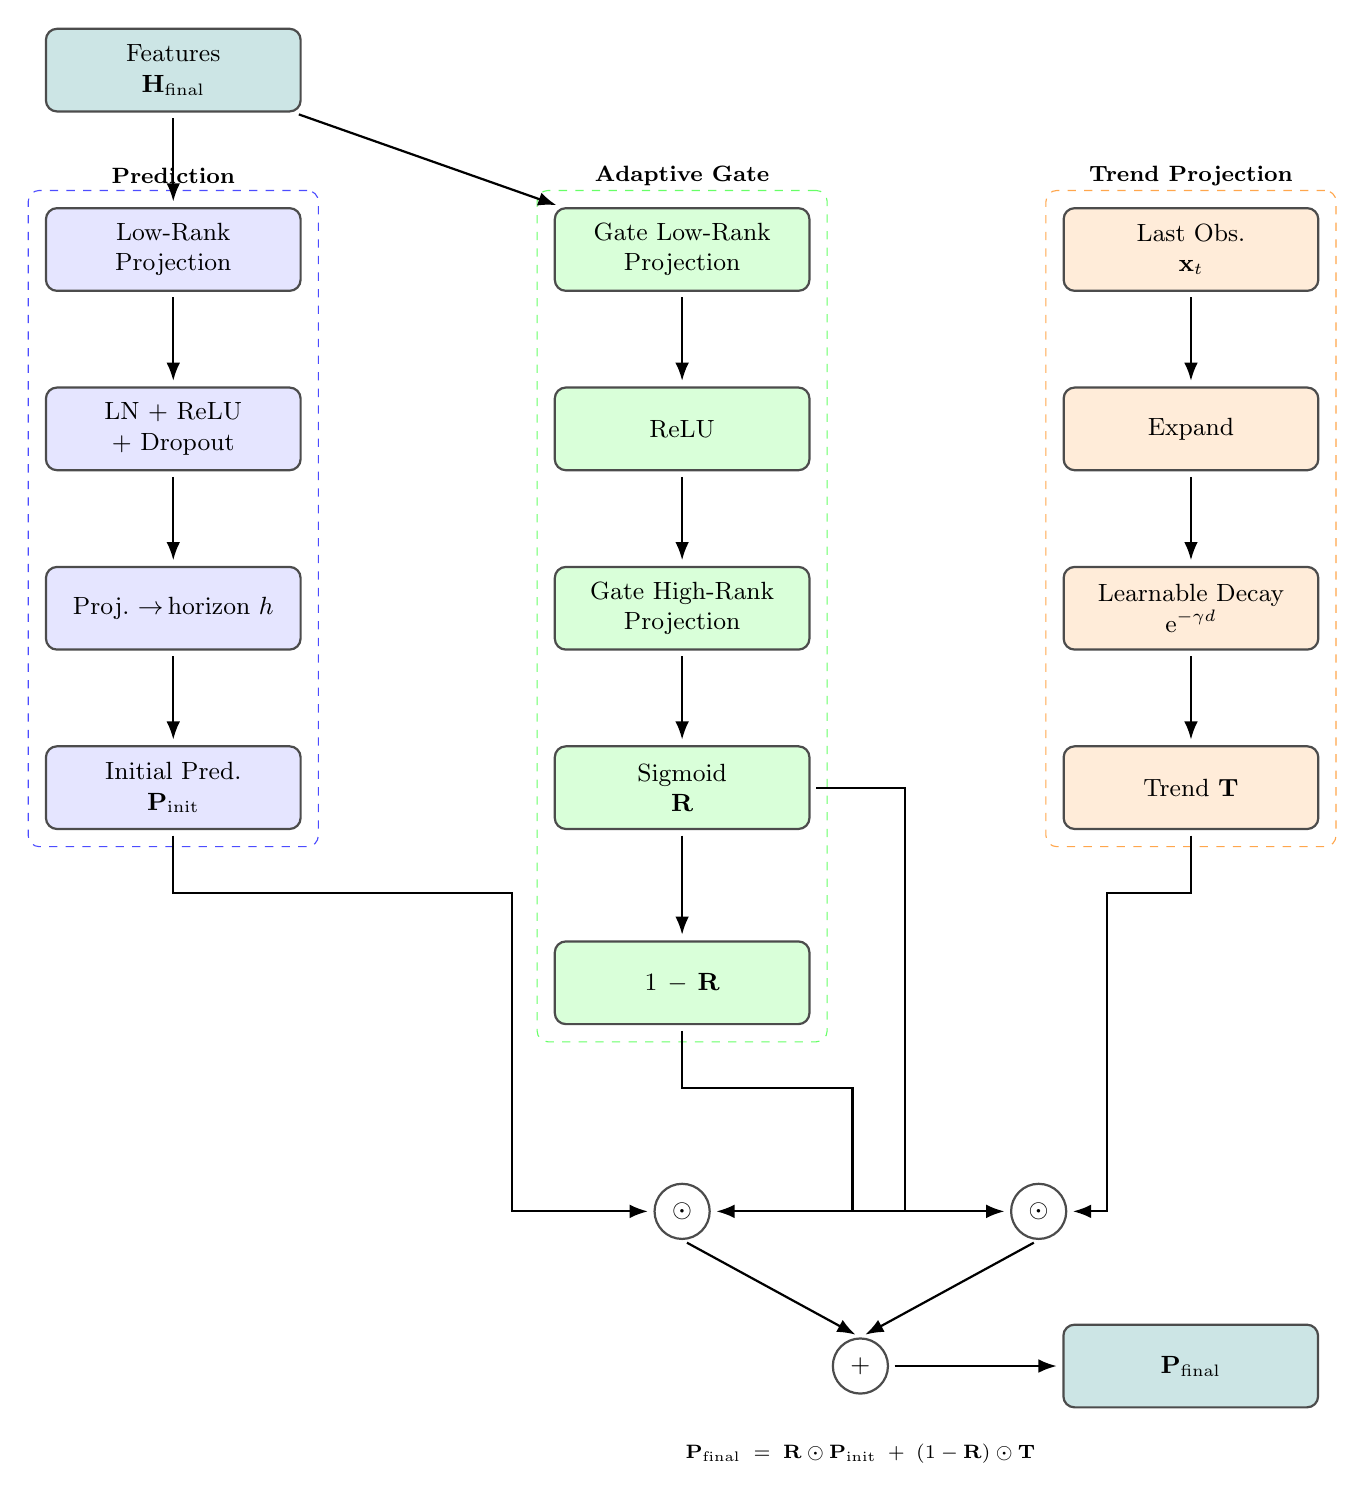
\begin{tikzpicture}[
    font=\small,
    >=Latex,
    node distance = 1.2cm and 1.8cm,
    block/.style={rectangle, draw=black!70, thick,
                  rounded corners, align=center,
                  minimum height=1.05cm, text width=3.0cm},
    pred/.style ={block, fill=blue!10},
    gate/.style ={block, fill=green!15},
    trend/.style={block, fill=orange!15},
    io/.style   ={block, fill=teal!20},
    op/.style   ={circle, draw=black!70, thick,
                  minimum size=0.7cm, inner sep=0pt},
    arrow/.style={->, thick, shorten >=2pt, shorten <=2pt}
]

%–––– INPUT –––––––––––––––––––––––––––––––––––––––––
\node (input) [io] {Features\\$\mathbf H_{\text{final}}$};

%–––– PREDICTION PATH ––––––––––––––––––––––––––––––
\node (plow)  [pred, below=of input]        {Low‑Rank\\Projection};
\node (pmid)  [pred, below=of plow]         {LN + ReLU + Dropout};
\node (phigh) [pred, below=of pmid]         {Proj. $\!\to\!$ horizon $h$};
\node (pinit) [pred, below=of phigh]        {Initial Pred.\\$\mathbf P_{\text{init}}$};

\foreach \a/\b in {input/plow, plow/pmid, pmid/phigh, phigh/pinit}
  \draw[arrow] (\a) -- (\b);

%–––– GATE PATH ––––––––––––––––––––––––––––––––––––
\node (glow)   [gate, right=3.2cm of plow]  {Gate Low‑Rank\\Projection};
\node (grelu)  [gate, below=of glow]        {ReLU};
\node (ghigh)  [gate, below=of grelu]       {Gate High‑Rank\\Projection};
\node (gsig)   [gate, below=of ghigh]       {Sigmoid\\$\mathbf R$};
\node (ginv)   [gate, below=1.4cm of gsig]  {$1-\mathbf R$};

\foreach \a/\b in {input/glow, glow/grelu, grelu/ghigh, ghigh/gsig, gsig/ginv}
  \draw[arrow] (\a) -- (\b);

%–––– TREND PATH –––––––––––––––––––––––––––––––––––
\node (last)   [trend, right=3.2cm of glow] {Last Obs.\\$\mathbf x_t$};
\node (expand) [trend, below=of last]       {Expand};
\node (decay)  [trend, below=of expand]     {Learnable Decay\\$\mathrm e^{-\gamma d}$};
\node (trend)  [trend, below=of decay]      {Trend $\mathbf T$};

\foreach \a/\b in {last/expand, expand/decay, decay/trend}
  \draw[arrow] (\a) -- (\b);

% FUSION OPS (now lower)
% Products placed well below group boxes
\node (mul1) [op, below=2.0cm of ginv] {$\odot$};
\node (mul2) [op, right=3.8cm of mul1] {$\odot$};

% Sum centred beneath the products
\node (add)  [op, below=1.6cm of $(mul1)!0.5!(mul2)$] {$+$};

\node (output) [io, right=2.2cm of add] {$\mathbf P_{\text{final}}$};

% Arrows from paths to products (entering from sides)
\draw[arrow] (pinit.south) -- ++ (0,-0.8) -| ($(mul1.west)+(-1.8,0)$) -- (mul1.west);
\draw[arrow] (gsig.east) -- ++ (1.2,0) |- (mul1.east);

\draw[arrow] (trend.south) -- ++ (0,-0.8) -| ($(mul2.east)+(0.5,0)$) -- (mul2.east);
\draw[arrow] (ginv.south) -- ++ (0,-0.8) -| ($(mul2.west)+(-2.0,0)$) -- (mul2.west);

% Products to sum, sum to output - direct connections are fine
\draw[arrow] (mul1.south) -- ($(mul1.south)!0.5!(add.north)$) -- (add.north);
\draw[arrow] (mul2.south) -- ($(mul2.south)!0.5!(add.north)$) -- (add.north);
\draw[arrow] (add.east) -- (output.west);

% EQUATION
\node (eq) [below=0.5cm of add, font=\scriptsize, align=center]
{$\displaystyle \mathbf P_{\text{final}}\;=\;
        \mathbf R \odot \mathbf P_{\text{init}}
        \;+\;
        (1-\mathbf R) \odot \mathbf T$};

% GROUP BOXES
\begin{scope}[on background layer]
  \node[draw=blue!70,  dashed, rounded corners, inner sep=6pt,
        fit=(plow)(pmid)(phigh)(pinit)] {};
  \node at ($(plow.north)+(0,0.4)$) [font=\footnotesize\bfseries] {Prediction};

  \node[draw=green!60, dashed, rounded corners, inner sep=6pt,
        fit=(glow)(grelu)(ghigh)(gsig)(ginv)] {};
  \node at ($(glow.north)+(0,0.4)$) [font=\footnotesize\bfseries] {Adaptive Gate};

  \node[draw=orange!70, dashed, rounded corners, inner sep=6pt,
        fit=(last)(expand)(decay)(trend)] {};
  \node at ($(last.north)+(0,0.4)$) [font=\footnotesize\bfseries] {Trend Projection};
\end{scope}
\end{tikzpicture}}%
% \caption{The flow of data in the PPRM architecture}
\caption{Data flow in the PPRM module. Features are projected through a low-rank bottleneck to generate initial predictions. An adaptive gate learns to balance these model-based forecasts with exponential trend extrapolations based on recent observations.}
\label{fig:pprm_module}
\end{figure}

\subsection{Highway Autoregressive Connection}

The final output of MSAGAT-Net blends the model's spatiotemporal predictions with a simple autoregressive baseline via a learnable highway connection. Given the last $w_h$ observations (with $w_h = \min(4, w)$), we compute a linear autoregressive forecast:

\begin{equation}
\mathbf{Z}_{\text{ar}} = \text{Linear}(\mathbf{X}_{[t-w_h+1:t]})
\end{equation}

where $\text{Linear}: \mathbb{R}^{w_h} \to \mathbb{R}^{h}$ projects recent observations to the forecast horizon for each region. The final prediction is a sigmoid-gated blend:

\begin{equation}
\hat{\mathbf{Y}} = \sigma(\lambda) \cdot \mathbf{P}_{\text{final}} + (1 - \sigma(\lambda)) \cdot \mathbf{Z}_{\text{ar}}
\end{equation}

where $\mathbf{P}_{\text{final}}$ is the PPRM output, $\lambda$ is a learnable scalar initialised to $0.5$, and $\sigma$ denotes the sigmoid function. This highway mechanism provides a direct gradient path from input to output, stabilises early training by anchoring predictions to recent observations, and allows the model to gracefully degrade to a simple autoregressive baseline when the learned spatiotemporal features are uninformative.

\section{Experimental Setup}
\label{sec:experiments}

We evaluate MSAGAT-Net against strong baselines on six epidemic datasets spanning influenza, COVID-19 case counts, and ICU bed occupancy, using root mean square error (RMSE), Pearson correlation coefficient (PCC), mean absolute error (MAE), and coefficient of determination (R\textsuperscript{2}).

\subsection{Computing Environment}
\label{sec:experimental_setup}

%All experiments were conducted on a high-performance computing (HPC) cluster equipped with Intel Xeon Gold 5217 @ 3.00\,GHz CPUs and NVIDIA RTX 8000 GPUs, ensuring consistent hardware conditions across all model evaluations.
All experiments were conducted on a desktop workstation equipped with an AMD Ryzen 7 7700 8-core processor (3.80\,GHz), 32\,GB DDR5 RAM, and an NVIDIA GeForce RTX 5060 Ti GPU (16\,GB GDDR7), ensuring consistent hardware conditions across all model evaluations.

\subsection{Datasets}
\label{sec:datasets}

To comprehensively evaluate the performance and generalisability of our proposed MSAGAT-Net framework, we performed experiments on several real-world epidemic datasets spanning various geographical regions, time periods, and disease types. This approach enables a thorough assessment of the model's versatility and robustness across varying spatiotemporal characteristics and epidemic scenarios.

Our experimental evaluation encompasses six distinct datasets, each offering unique challenges and characteristics for epidemic forecasting. These datasets represent different geographical scales (from local authorities to national regions), temporal resolutions (daily and weekly measurements), and disease contexts (seasonal influenza and COVID-19). Table~\ref{tab:datasets} provides a statistical overview of these datasets, summarising their key characteristics and numerical properties.

\begin{table}[!htbp]
\centering
\caption{Overview of the epidemic datasets used in our experimental evaluation. ``Granularity'' indicates the temporal resolution of the epidemic data, whilst ``Size'' represents the product of the number of locations and the number of time steps.}
\label{tab:datasets}
\begin{tabular}{lccccc}
\hline
\textbf{Dataset} & \textbf{Size} & \textbf{Min} & \textbf{Max} & \textbf{Mean} & \textbf{Granularity} \\
\hline
Japan-Prefecture & $348 \times 47$ & 0 & 26,635 & 655 & Weekly \\
US-Region & $785 \times 10$ & 0 & 16,526 & 1,009 & Weekly \\
US-State & $360 \times 49$ & 0 & 9,716 & 223 & Weekly \\
Australia-COVID & $556 \times 8$ & 0 & 9,987 & 539 & Daily \\
LTLA-COVID & $839 \times 372$ & 0 & 4,170 & 85 & Daily \\
NHS-ICUBeds & $895 \times 7$ & 0 & 1,215 & 102 & Daily \\
\hline
\end{tabular}
\end{table}

\subsubsection{Influenza Datasets}
We used three established influenza datasets from different regions to evaluate our model's performance on seasonal patterns:

\begin{itemize}
    \item \textbf{Japan-Prefecture Dataset:} This dataset is derived from the Infectious Disease Weekly Report (IDWR) published by the Japanese government\footnote{\url{https://tinyurl.com/y5dt7stm}}. It comprises weekly statistics of ILI cases from August 2012 to March 2019 in all 47 prefectures in Japan. 
    
    \item \textbf{US-Region Dataset:} Extracted from the ILINet surveillance system maintained by the US Health and Human Services (US-HHS)\footnote{\url{https://tinyurl.com/y39tog3h}}, this dataset includes weekly influenza activity levels in ten HHS regions across the continental United States from 2002 to 2017. 

    \item \textbf{US-State Dataset:} Obtained from the Centres for Disease Control and Prevention (CDC), this dataset consists of weekly numbers of visits to healthcare providers with influenza-like illnesses from 2010 to 2017 for 49 states in the US (one state was excluded due to incomplete data).
\end{itemize}

\subsubsection{COVID-19 Datasets}
To assess the adaptability of our model to new epidemic scenarios, we incorporated three COVID-19 datasets that span different countries and healthcare metrics:

\begin{itemize}
    \item \textbf{Australia-COVID Dataset:} Compiled from the Johns Hopkins University Centre for Systems Science and Engineering (JHU-CSSE) repository, this dataset contains daily new confirmed cases of COVID-19 from 27 January 2020 to 4 August 2021 across all eight Australian jurisdictions (six states and two territories).

    \item \textbf{LTLA-COVID Dataset:} Derived from the UK Health Security Agency\footnote{\url{https://ukhsa-dashboard.data.gov.uk/respiratory-viruses/covid-19}}, this dataset contains daily data from COVID-19 cases from March 2020 to February 2022 for 372 Lower-Tier Local Authority districts in England. We constructed spatial graph structures for this dataset using geographic proximity, providing a spatiotemporal benchmark for COVID-19 forecasting at the local authority level.
    
    \item \textbf{NHS-ICUBeds Dataset:} Obtained from the National Health Service (NHS) England\cite{NHS2024HospitalActivity}, this dataset provides daily counts of mechanical ventilator beds occupied in seven regions of the NHS from March 2020 to February 2022. Unlike the other datasets that focus on case counts, this dataset offers an opportunity to evaluate the model's capability to predict healthcare resource utilisation, which is critical for effective epidemic response and management. We constructed spatial connectivity structures for this dataset, addressing the gap in spatially-structured healthcare resource forecasting benchmarks.
\end{itemize}

\subsection{Spatial Graph Construction}
\label{sec:graph_construction} 

Following the established methodology of STAN \cite{gao2021stan}, we construct spatial graph structures to capture epidemic transmission patterns between geographic regions using geographic proximity as the primary criterion for establishing spatial relationships. For the LTLA-COVID and NHS-ICUBeds datasets, which previously lacked predefined spatial connectivity structures, we developed these spatial graphs to enable spatiotemporal modeling of these publicly available epidemic data sources.

For our implementation, we constructed the adjacency matrix based on geographic proximity, using the Haversine formula to calculate the great circle distance between regions, consistent with established practices in spatiotemporal epidemic modelling. Two regions are considered connected if the distance between them falls below a threshold $d_{\text{threshold}}$ (set to 150 km in our experiments):

\begin{equation}
a_{ij} = 
\begin{cases}
1, & \text{if } \text{Haversine}(\text{region}_i, \text{region}_j) \leq d_{\text{threshold}} \\
0, & \text{otherwise}
\end{cases}
\end{equation}

This threshold-based connectivity captures the intuition that epidemic spread is influenced by the movement of people between nearby regions. Although more sophisticated connectivity measures could be employed, this approach provides a straightforward and interpretable baseline for spatial relationship modelling. The noise in the dataset was smoothed using the rolling mean of 7 days established in previous studies \cite{ajao2023deep, oluwasakin2023data, zeroual2020deep, Kamalov2022ReviewDL}, and normalisation was performed to ensure that the data are on a similar scale in different regions.

The diverse nature of these datasets, spanning different geographic regions, temporal resolutions, and epidemic contexts, allows us to comprehensively evaluate the performance and generalisability of our proposed MSAGAT-Net model across a range of epidemic forecasting scenarios.

\subsection{Training and Optimisation Strategy}
\label{sec:optimisation}

The MSAGAT-Net model is trained using the Adam optimiser with a learning rate of $1 \times 10^{-3}$ and a batch size of 32, which were determined through preliminary hyperparameter tuning to provide optimal convergence speed and stability. The model is trained for a maximum of 1500 epochs, with early stopping criteria based on validation loss to prevent overfitting. The training process is monitored using a patience parameter of 100 epochs, which means that if the validation loss does not improve for 100 consecutive epochs, the training will be stopped. The loss function for the MSAGAT-Net model is a combination of forecast error and regularisation terms:

\begin{equation}
\label{eq:total_loss}
\mathcal{L}_{\text{total}} = \mathcal{L}_{\text{forecast}} + \lambda_{\text{attn}}\mathcal{L}_{\text{attn}} + \lambda_{\text{l2}}\|\Theta\|_2
\end{equation}

where $\mathcal{L}_{\text{forecast}}$ is the mean squared error measuring discrepancies between the model forecasts and the observed data, and $\mathcal{L}_{\text{attn}}$ represents the attention regularisation term that enforces sparsity and interpretability in spatial relationships. The hyperparameters $\lambda_{\text{attn}}$ and $\lambda_{\text{l2}}$ control the strength of attention and L2 regularisation, respectively. Following prior work on graph attention and spatiotemporal forecasting networks \cite{velickovic2017graph, zhang2019spatial, xie2022epignn, dengColaGNNCrosslocationAttention2020a, wang2020linformer}, we initialise $\lambda_{\text{attn}}$ at $10^{-5}$ and optimise it as a learnable parameter during training, allowing the model to adaptively balance forecast accuracy with attention sparsity. In contrast, $\lambda_{\text{l2}} = 5 \times 10^{-4}$ remains fixed throughout training, consistent with established practices that balance generalisation and numerical stability.

For all datasets, we employ a sliding window of 20 time steps and split the data into training, validation, and test sets with a ratio of 60\%:20\%:20\%. The complete training procedure is formalised in Algorithm~\ref{alg:MSAGAT-Net_training}. Table~\ref{tab:hyperparameters} summarises all architectural hyperparameters.

\begin{table}[!htbp]
\centering
\caption{MSAGAT-Net architectural hyperparameters. All values are shared across datasets. Parameters marked $^\dagger$ are learnable; the listed value is the initialisation.}
\label{tab:hyperparameters}
\begin{tabular}{@{}llr@{}}
\toprule
\textbf{Module} & \textbf{Hyperparameter} & \textbf{Value} \\
\midrule
\multirow{4}{*}{TFEM}
 & Feature channels $d_{\text{feat}}$ & 16 \\
 & Kernel size & 3 \\
 & Bottleneck dim $d_{\text{bottle}}$ & 8 \\
 & Hidden dim $d_{\text{hidden}}$ & 32 \\
\midrule
\multirow{4}{*}{EAGAM}
 & Attention heads & 4 \\
 & Bottleneck dim $d_{\text{bottle}}$ & 8 \\
 & Attn.\ reg.\ weight $\lambda_{\text{attn}}^{\dagger}$ & $10^{-5}$ \\
 & Adj.\ prior scale $\alpha_0^{\dagger}$ & 1.0 \\
\midrule
MSSFM & Max hops $S_{\max}$ & 4 \\
\midrule
\multirow{3}{*}{PPRM}
 & Bottleneck dim $d_{\text{bottle}}$ & 8 \\
 & Decay $\gamma_0^{\dagger}$ & $-2.3$ \\
 & Dropout & 0.2 \\
\midrule
\multirow{2}{*}{Highway}
 & Window $w_h$ & $\min(4, w)$ \\
 & Gate $\lambda^{\dagger}$ & 0.5 \\
\bottomrule
\end{tabular}
\end{table}

\begin{algorithm}[!ht]
    \caption{MSAGAT-Net Training Algorithm}
    \label{alg:MSAGAT-Net_training}
    \KwIn{Training data $\mathcal{D}_{\text{train}}$, validation data $\mathcal{D}_{\text{val}}$}
    \KwOut{Optimized model parameters $\boldsymbol{\Theta}^*$}
    
    Initialize model parameters $\boldsymbol{\Theta}$ (including graph bias $\mathbf{U}, \mathbf{V}$) and Adam optimizer with weight decay $\lambda_{\text{l2}}$\;
    $L_{\text{best}} \leftarrow \infty$, $p \leftarrow 0$ \tcp*{Best validation loss and patience counter}
    
    \For{epoch $e = 1$ \KwTo $E_{\max}$}{
      \ForEach{mini-batch $(\mathbf{X}, \mathbf{y})$ in $\mathcal{D}_{\text{train}}$}{
        
        $\mathbf{F} \leftarrow \text{TFEM}(\mathbf{X})$ \tcp*{Depthwise sep. conv + bottleneck}
        
        $\mathbf{G}, \mathcal{L}_{\text{attn}} \leftarrow \text{EAGAM}(\mathbf{F})$ \tcp*{Scaled dot-product + structural bias}
        
        $\mathbf{H} \leftarrow \text{MSSFM}(\mathbf{G})$ \tcp*{Multi-hop graph conv + fusion}
        
        $\mathbf{P} \leftarrow \text{PPRM}(\mathbf{H}, \mathbf{x}_{\text{last}})$ \tcp*{Progressive refinement}
        
        $\mathbf{Z}_{\text{ar}} \leftarrow \text{Linear}(\mathbf{X}_{[t-w_h+1:t]})$ \tcp*{Autoregressive baseline}
        $\hat{\mathbf{Y}} \leftarrow \sigma(\lambda)\mathbf{P} + (1-\sigma(\lambda))\mathbf{Z}_{\text{ar}}$ \tcp*{Highway blend}
        
        $\mathcal{L}_{\text{total}} \leftarrow \mathcal{L}_{\text{MSE}}(\hat{\mathbf{Y}}, \mathbf{y}) + \mathcal{L}_{\text{attn}}$ \tcp*{L2 handled by optimizer}
        
        Update $\boldsymbol{\Theta}$ using gradient descent on $\mathcal{L}_{\text{total}}$\;
      }
      
      $L_{\text{val}} \leftarrow \text{Evaluate}(\mathcal{D}_{\text{val}}, \boldsymbol{\Theta})$ \tcp*{Compute validation loss}
      
      \eIf{$L_{\text{val}} < L_{\text{best}}$}{
        $\boldsymbol{\Theta}^* \leftarrow \boldsymbol{\Theta}$, $L_{\text{best}} \leftarrow L_{\text{val}}$, $p \leftarrow 0$\;
      }{
        $p \leftarrow p + 1$\;
        \If{$p \geq P_{\text{max}}$}{
          \textbf{break}\;
        }
      }
    }
    \KwRet{$\boldsymbol{\Theta}^*$}
\end{algorithm}



\subsection{Baseline Models}
\label{sec:baseline_models}

We compare MSAGAT-Net against several state-of-the-art baseline models widely used in epidemic forecasting:

\begin{itemize}
    \item \textbf{DCRNN}~\cite{li2017diffusion}: A diffusion convolution recurrent neural network that integrates graph convolutions with recurrent neural networks in an encoder-decoder architecture to capture both spatial dependencies and temporal dynamics. It models spatial dependencies using a diffusion process on graphs and temporal dependencies through recurrent units. \textit{Requires a predefined adjacency matrix to perform diffusion convolutions.}
    
    \item \textbf{LSTNet}~\cite{lai2018modeling}: A model that combines convolutional neural networks and recurrent neural networks to extract short-term local dependency patterns and discover long-term patterns for time-series trends. It employs a convolutional component to extract local dependency patterns and a recurrent component to capture long-term temporal dependencies. \textit{Does not model explicit spatial structure.}
    
    \item \textbf{CNNRNN-Res}~\cite{wu2018deep}: A deep learning framework that combines convolutional neural networks, recurrent neural networks, and residual connections to solve epidemiological prediction problems. It uses CNNs to extract spatial features, RNNs to capture temporal dependencies, and residual connections to enhance gradient flow during training. \textit{Does not model explicit spatial structure.}
    
    \item \textbf{Cola-GNN}~\cite{dengColaGNNCrosslocationAttention2020a}: A graph neural network model that leverages cross-location attention mechanisms to capture dynamic spatial relationships between regions. It employs location-aware attention to model the impact of each region on others, allowing for adaptive and context-dependent spatial dependency learning. \textit{Requires a predefined adjacency matrix to initialise and constrain the attention mechanism.}
    
    \item \textbf{EpiGNN}~\cite{xie2022epignn}: A model based on graph neural networks specifically designed for epidemic forecasting. It incorporates a transmission risk encoding module to characterise local and global spatial effects, and features a Region-Aware Graph Learner (RAGL) that considers transmission risk, geographical dependencies, and temporal information to explore spatiotemporal dependencies. \textit{Requires a predefined adjacency matrix (specified via the \texttt{--sim\_mat} parameter) to encode geographical dependencies.}
\end{itemize}

These baselines represent a diverse range of approaches to spatiotemporal forecasting. A key distinction is that all graph-based baselines (DCRNN, Cola-GNN, EpiGNN) require predefined adjacency matrices as mandatory input, whereas MSAGAT-Net learns spatial relationships through learnable graph bias parameters $\mathbf{U}$ and $\mathbf{V}$ and can optionally incorporate adjacency as a self-regulating soft prior (Section~\ref{sec:adj_prior}). In our experiments, MSAGAT-Net uses the adjacency prior when available, but ablation results (Section~\ref{sec:results}) confirm competitive performance without it.

\section{Results and Discussion}
\label{sec:results}

Table~\ref{tab:performance_table} presents a comprehensive comparison of our proposed MSAGAT-Net model against state-of-the-art baseline approaches across three influenza datasets (Japan-Prefectures, US-Regions, and US-States) and four forecast horizons (3, 5, 10, and 15 days ahead). Furthermore, Table~\ref{tab:performance_table_others} shows the performance comparison on three COVID-19 datasets (Australia-COVID, LTLA-TimeSeries, and NHS-TimeSeries) for horizons of 3, 7, and 14 days ahead.

\begin{table}[!ht]
    \centering
    \caption{RMSE and PCC performance of different methods on three datasets (horizon = 3, 5, 10, 15). Bold = best, underline = second best.}
    \label{tab:performance_table}
    \resizebox{\textwidth}{!}{%
    \begin{tabular}{llrrrrrrrrrrrr}
        \toprule
        \multirow{2}{*}{Method} & \multirow{2}{*}{Metric}
            & \multicolumn{4}{c}{Japan–Prefectures}
            & \multicolumn{4}{c}{US–Regions}
            & \multicolumn{4}{c}{US–States} \\
        \cmidrule(lr){3-6} \cmidrule(lr){7-10} \cmidrule(lr){11-14}
         &  & 3 & 5 & 10 & 15 & 3 & 5 & 10 & 15 & 3 & 5 & 10 & 15 \\
        \midrule
        DCRNN       & RMSE & 2345 & 2610 & 2579 & 2284 & 1116 & 1381 & 1652 & 1666 & 235 & 292 & 340 & 366 \\
                    & PCC  & 0.424 & 0.238 & 0.555 & 0.515 & 0.791 & 0.684 & 0.573 & 0.565 & 0.899 & 0.843 & 0.823 & 0.804 \\
        \midrule
        LSTNet      & RMSE & 2360 & 2595 & 2470 & 1999 & 965 & 1139 & 1224 & \underline{1143} & 247 & 297 & 354 & 380 \\
                    & PCC  & 0.392 & 0.190 & 0.416 & 0.567 & 0.802 & 0.730 & 0.636 & 0.683 & 0.855 & 0.775 & 0.777 & 0.750 \\
        \midrule
        CNNRNN-Res  & RMSE & 2289 & 2653 & 2710 & 1943 & 874 & 1154 & 1373 & 1277 & 288 & 328 & 313 & 360 \\
                    & PCC  & 0.445 & 0.102 & 0.255 & 0.611 & 0.834 & 0.696 & 0.579 & 0.632 & 0.801 & 0.744 & 0.817 & 0.765 \\
        \midrule
        Cola-GNN    & RMSE & 1548 & 1772 & \underline{1802} & 1836 & 774 & 1030 & \textbf{888} & \textbf{1063} & 203 & 228 & 271 & 280 \\
                    & PCC  & \underline{0.845} & 0.798 & \underline{0.792} & 0.705 & 0.882 & 0.804 & \textbf{0.840} & \textbf{0.800} & 0.914 & 0.902 & \textbf{0.896} & \textbf{0.907} \\
        \midrule
        EpiGNN      & RMSE & \textbf{1272} & \underline{1647} & 1806 & \underline{1692} & \underline{689} & \underline{852} & 1169 & 1224 & \underline{187} & \underline{207} & \underline{240} & \underline{248} \\
                    & PCC  & \textbf{0.880} & \underline{0.813} & 0.724 & \underline{0.732} & \underline{0.898} & \textbf{0.860} & 0.723 & \underline{0.716} & \underline{0.923} & \textbf{0.907} & 0.884 & \underline{0.888} \\
        \midrule
        MSAGAT-Net & RMSE & \underline{1385} & \textbf{1437} & \textbf{1584} & \textbf{1550} & \textbf{659} & \textbf{902} & \underline{962} & 1334 & \textbf{163} & \textbf{197} & \textbf{226} & \textbf{245} \\
                    & PCC  & 0.836 & \textbf{0.852} & \textbf{0.831} & \textbf{0.816} & \textbf{0.907} & \underline{0.816} & \underline{0.800} & 0.562 & \textbf{0.936} & \underline{0.907} & \underline{0.885} & 0.876 \\
        \bottomrule
    \end{tabular}%
    }
\end{table}


\begin{table}[!ht]
    \centering
    \caption{RMSE and PCC performance of different methods on three COVID-19 datasets (horizon = 3, 7, 14). Bold = best, underline = second best.}
    \label{tab:performance_table_others}
    \resizebox{\textwidth}{!}{%
    \begin{tabular}{llrrrrrrrrrr}
        \toprule
        \multirow{2}{*}{Method} & \multirow{2}{*}{Metric}
            & \multicolumn{3}{c}{Australia-COVID}
            & \multicolumn{3}{c}{LTLA-Timeseries}
            & \multicolumn{3}{c}{NHS-Timeseries} \\
        \cmidrule(lr){3-5}\cmidrule(lr){6-8}\cmidrule(lr){9-11}
         &  & 3 & 7 & 14  & 3 & 7 & 14  & 3  & 7  & 14 \\
        \midrule
        DCRNN       & RMSE & 230 & 360 & 634 & 64.5 & \underline{109} & 145 & 5.10 & 9.07 & 15.7 \\
                    & PCC  & 0.996 & 0.985 & 0.972 & 0.908 & \underline{0.707} & 0.440 & 0.977 & 0.932 & 0.830 \\
        \midrule
        LSTNet      & RMSE & 367 & \textbf{248} & \textbf{298} & \underline{57.5} & 115 & 149 & 3.66 & 10.2 & 17.9 \\
                    & PCC  & 0.984 & \textbf{0.994} & \textbf{0.992} & \underline{0.927} & 0.663 & 0.430 & 0.988 & 0.907 & 0.669 \\
        \midrule
        CNNRNN-Res  & RMSE & \textbf{153} & \underline{300} & \underline{352} & 121 & 131 & \underline{140} & 4.20 & 9.77 & \textbf{13.0} \\
                    & PCC  & \underline{0.998} & 0.991 & 0.986 & 0.612 & 0.528 & 0.449 & 0.984 & 0.942 & 0.844 \\
        \midrule
        Cola-GNN    & RMSE & 265 & 362 & 575 & 70.6 & 247 & 143 & \textbf{3.15} & 9.56 & 14.2 \\
                    & PCC  & 0.997 & 0.993 & 0.985 & 0.886 & 0.164 & \underline{0.453} & \underline{0.991} & \underline{0.945} & 0.840 \\
        \midrule
        EpiGNN      & RMSE & 318 & 387 & 463 & 155 & 144 & 157 & 6.74 & \underline{8.11} & \underline{13.2} \\
                    & PCC  & 0.995 & 0.992 & \underline{0.987} & 0.530 & 0.501 & 0.448 & 0.962 & 0.944 & \textbf{0.869} \\
        \midrule
        MSAGAT-Net & RMSE & \underline{226} & 372 & 650 & \textbf{49.8} & \textbf{83.0} & \textbf{116} & \underline{3.45} & \textbf{6.31} & 13.9 \\
                    & PCC  & \textbf{0.998} & \underline{0.994} & 0.986 & \textbf{0.945} & \textbf{0.842} & \textbf{0.653} & \textbf{0.993} & \textbf{0.965} & \underline{0.869} \\
        \bottomrule
    \end{tabular}%
    }
\end{table}

\subsubsection{Performance on Influenza Datasets}

The Japan-Prefectures dataset provides strong validation of MSAGAT-Net's architectural design. Whilst EpiGNN achieves the best short-term performance (3-day RMSE: 1272), MSAGAT-Net delivers the best results for medium- and long-term horizons (5-day RMSE: 1437, 10-day: 1584, 15-day: 1550), consistently outperforming all baselines from horizon 5 onwards. MSAGAT-Net also achieves the highest correlation coefficients at these extended horizons (PCC: 0.852, 0.831, 0.816), demonstrating that the model's learnable graph structure, additive structural-bias attention, and multi-hop spatial refinement effectively capture the complex spatiotemporal dynamics of influenza transmission between Japanese prefectures, particularly for longer-range forecasting where spatial dependencies become increasingly important.

The attention visualisation in Figure~\ref{fig:attention_matrices_none} reveals why MSAGAT-Net succeeds on this dataset: the learned attention patterns diverge substantially from both geographical adjacency and simple correlation structures, identifying epidemic-relevant connections that likely reflect commuter flows, air travel routes, and socioeconomic linkages rather than mere proximity. This data-driven discovery of transmission pathways, enabled by the learnable graph bias parameters ($\mathbf{U}$, $\mathbf{V}$), represents a key advantage over baselines that rely on predefined spatial structures.

Performance on US-Regions and US-States reveals nuanced patterns. On US-Regions, MSAGAT-Net achieves the best short-term RMSE (3-day: 659) and competitive 5-day performance (902), whilst Cola-GNN dominates at longer horizons (10-day: 888, 15-day: 1063). On US-States, MSAGAT-Net achieves the best RMSE across all four horizons (3-day: 163, 5-day: 197, 10-day: 226, 15-day: 245), consistently outperforming EpiGNN and Cola-GNN. However, PCC analysis reveals that Cola-GNN achieves the highest correlation for 10-day and 15-day US-States forecasts (0.896, 0.907), suggesting that when explicit graph structure is available, Cola-GNN's attention mechanism can produce better-correlated predictions even when absolute errors are higher. The US-Regions 15-day horizon remains a weakness (RMSE: 1334, PCC: 0.562), likely due to the small node count (10 regions) limiting the benefit of MSAGAT-Net's adaptive multi-hop spatial learning.

\subsubsection{Performance on COVID-19 Datasets}

COVID-19 datasets reveal context-dependent performance patterns that illuminate the conditions under which MSAGAT-Net's architectural choices confer advantages. On LTLA-Timeseries (372 nodes, highest spatial resolution), MSAGAT-Net achieves the best performance across all horizons (3-day RMSE: 49.8, 7-day: 83.0, 14-day: 116), substantially outperforming all baselines. The improvements are particularly striking: 13.5\% lower RMSE than LSTNet (second-best) at 3-day, 23.5\% lower than DCRNN (second-best) at 7-day, and 17.3\% lower than CNNRNN-Res (second-best) at 14-day. MSAGAT-Net also achieves the highest PCC across all horizons (0.945, 0.842, 0.653), confirming that structural-bias attention and multi-hop spatial refinement are highly effective at larger spatial scales where the graph structure encodes meaningful transmission patterns between local authorities.

The Australia-COVID dataset (8 nodes, 556 timesteps) reveals a different dynamic. CNNRNN-Res achieves the best 3-day RMSE (153), whilst LSTNet dominates at 7-day (248) and 14-day (298) horizons. MSAGAT-Net performs competitively (3-day RMSE: 226, second-best) but falls behind at longer horizons (7-day: 372, 14-day: 650). This pattern is informative: Australia's COVID-19 response involved strict state border closures and aggressive containment, effectively decoupling spatial transmission. With only 8 nodes and minimal inter-regional coupling, the dataset offers insufficient spatial complexity to benefit from graph-based modelling. The success of simpler models (LSTNet, CNNRNN-Res) confirms that purely temporal approaches are optimal when spatial dependencies are suppressed by policy interventions.

On NHS-Timeseries (7 nodes, ICU bed occupancy), MSAGAT-Net achieves the best RMSE at 7-day (6.31) and strong performance at the other horizons: 3-day RMSE 3.45 (second to Cola-GNN's 3.15) and 14-day RMSE 13.9 (competitive with CNNRNN-Res's 13.0 and EpiGNN's 13.2). MSAGAT-Net achieves the highest PCC at 3-day (0.993) and 7-day (0.965), whilst EpiGNN leads at 14-day (0.869 vs 0.869, effectively tied). This strong performance on a very small graph (7 nodes) suggests that MSAGAT-Net's adaptive architecture effectively handles both large and small spatial scales, leveraging temporal dynamics when spatial complexity is limited. The shift from case counts to resource utilisation introduces different temporal dynamics (administrative delays, capacity constraints), but MSAGAT-Net's progressive prediction refinement module appears well-suited to capture these patterns.

\subsubsection{Synthesis: When MSAGAT-Net Succeeds}

Cross-dataset analysis reveals that MSAGAT-Net achieves the best or second-best RMSE in the majority of experimental settings across all six datasets. The model dominates on LTLA-Timeseries (best at all horizons), US-States (best RMSE at all four horizons), and Japan-Prefectures (best from 5-day onward), with strong performance on NHS-Timeseries (best at 7-day, competitive at 3- and 14-day). This demonstrates strong generalisation across both influenza and COVID-19 contexts. Performance is weakest on Australia-COVID, where the combination of few nodes (8) and suppressed spatial coupling due to border closures limits the benefit of graph-based spatial learning. The consistent strength on datasets with moderate-to-large spatial scale (47--372 nodes) confirms that MSAGAT-Net's adaptive spatial learning and multi-hop refinement are most effective when sufficient spatial complexity exists to discover meaningful transmission pathways.

\subsubsection{Qualitative Forecast Analysis}

Figure~\ref{fig:predictions_summary} presents an aggregated view of MSAGAT-Net's forecasting performance across all six datasets, showing the mean prediction across all regions with $\pm 1$ standard deviation confidence bands (left panels) and the temporal distribution of absolute prediction errors (right panels). Across all datasets, the predicted mean closely follows the ground truth, with narrow error bands during quiescent periods and wider bands during epidemic peaks---consistent with the inherent difficulty of forecasting rapid case surges. The model accurately tracks sharp seasonal peaks in Japan-Prefectures and US-States influenza, irregular COVID-19 waves in Australia and LTLA, and ICU bed occupancy patterns in NHS-Timeseries. The error plots reveal that prediction errors are temporally concentrated around peak periods rather than uniformly distributed, suggesting that MSAGAT-Net captures the overall epidemic trajectory well but faces challenges during the most dynamic phases of outbreaks. The close correspondence between predicted and actual values confirms that the quantitative improvements reported in Tables~\ref{tab:performance_table} and~\ref{tab:performance_table_others} translate into visually meaningful forecast quality.

\begin{figure}[!ht]
  \centering
  \begin{minipage}{0.49\linewidth}
    \centering
    \subfloat[Japan-Prefectures (5-day)]{
      \includegraphics[width=\linewidth]{msagat_figs/predictions_summary_japan_h5.png}%
      \label{fig:predsumm_japan}
    }
  \end{minipage}\hfill
  \begin{minipage}{0.49\linewidth}
    \centering
    \subfloat[US-Regions (5-day)]{
      \includegraphics[width=\linewidth]{msagat_figs/predictions_summary_region785_h5.png}%
      \label{fig:predsumm_region}
    }
  \end{minipage}

  \vspace{0.4em}

  \begin{minipage}{0.49\linewidth}
    \centering
    \subfloat[US-States (5-day)]{
      \includegraphics[width=\linewidth]{msagat_figs/predictions_summary_state360_h5.png}%
      \label{fig:predsumm_state}
    }
  \end{minipage}\hfill
  \begin{minipage}{0.49\linewidth}
    \centering
    \subfloat[Australia-COVID (7-day)]{
      \includegraphics[width=\linewidth]{msagat_figs/predictions_summary_australia-covid_h7.png}%
      \label{fig:predsumm_australia}
    }
  \end{minipage}

  \vspace{0.4em}

  \begin{minipage}{0.49\linewidth}
    \centering
    \subfloat[LTLA-Timeseries (7-day)]{
      \includegraphics[width=\linewidth]{msagat_figs/predictions_summary_ltla_timeseries_h7.png}%
      \label{fig:predsumm_ltla}
    }
  \end{minipage}\hfill
  \begin{minipage}{0.49\linewidth}
    \centering
    \subfloat[NHS-Timeseries (7-day)]{
      \includegraphics[width=\linewidth]{msagat_figs/predictions_summary_nhs_timeseries_h7.png}%
      \label{fig:predsumm_nhs}
    }
  \end{minipage}

  \caption{Aggregated prediction performance across all regions for each dataset. Left panels: mean prediction (red dashed) vs.\ ground truth (blue solid) with $\pm 1$ standard deviation bands. Right panels: temporal distribution of absolute prediction errors, showing that errors concentrate around epidemic peaks.}
  \label{fig:predictions_summary}
\end{figure}

\subsubsection{Learned Spatial Representations}

Figures~\ref{fig:attention_matrices_none}, \ref{fig:attention_matrices_no_pprm}, and \ref{fig:attention_matrices_no_eagam} provide visual evidence of EAGAM's role in discovering epidemic-relevant spatial structure. The complete model (Figure~\ref{fig:attention_matrices_none}) learns attention patterns that exhibit three key characteristics: (1) strong diagonal dominance indicating local temporal persistence, (2) structured off-diagonal patterns capturing inter-prefectural dependencies, and (3) substantial divergence from both geographical adjacency (left panel) and simple input correlation (center panel). This divergence is critical---it demonstrates that EAGAM does not merely replicate predefined structures but discovers latent transmission pathways informed by actual epidemic dynamics rather than geographic or statistical proxies.

Qualitatively, the learned attention matrix shows low similarity to the adjacency matrix, suggesting that epidemic transmission does not align with simple geographical proximity in modern Japan where bullet trains, air travel, and economic corridors create complex mobility patterns. The attention patterns reveal long-range connections between major metropolitan areas (Tokyo, Osaka, Nagoya) that would be missed by adjacency-based methods, whilst also capturing local clustering in rural prefectures---a nuanced spatial structure that emerges from the data rather than being imposed a priori.

The ablation variants confirm EAGAM's architectural necessity. Removing PPRM (Figure~\ref{fig:attention_matrices_no_pprm}) produces nearly identical attention patterns, validating that PPRM operates on prediction refinement rather than spatial learning---the attention mechanism remains intact because EAGAM is preserved. In stark contrast, removing EAGAM (Figure~\ref{fig:attention_matrices_no_eagam}) forces the model to use an identity spatial module (diagonal pattern in right panel), where each prefecture attends only to itself with zero inter-regional information flow. This ablation variant replaces EAGAM with a minimal identity pass-through (see Section~\ref{sec:ablation}), eliminating all spatial dependency modelling. The ablation results (Table~\ref{tab:ablation}) show that EAGAM removal produces consistent degradation across all horizons, with the strongest impact at 7-day (+17.11\% RMSE, $-$22.47\% R\textsuperscript{2}), confirming that adaptive spatial attention is the most critical component of MSAGAT-Net.

These visualisations collectively demonstrate that EAGAM's learnable graph bias mechanism ($\mathbf{B} = \mathbf{UV}$ with low-rank factorisation) successfully discovers and exploits non-obvious spatial relationships that predefined adjacency matrices alone cannot capture. Notably, the magnitude of the learned graph bias varies across datasets: on Japan-Prefectures, $\mathbf{B}$ develops pronounced structure reflecting inter-prefectural transmission pathways, whereas on datasets where content-based attention ($\mathbf{QK}^{\!\top}$) and the adjacency prior already capture the dominant spatial dependencies, the graph bias remains near its initialisation. This behaviour reflects the model's ability to adaptively allocate representational capacity---relying more on structural bias when data-driven spatial relationships are informative, and defaulting to content-based attention when they are not. This capability is particularly valuable for epidemic forecasting where true transmission networks rarely align with administrative boundaries or simple proximity measures.

\begin{figure}[h]
  \centering
  \includegraphics[width=0.9\textwidth]{msagat_figs/matrices_MSAGAT-Net.japan.w-20.h-7.none.png}
  \caption{Attention matrices learned by MSAGAT-Net on the Japan-Prefectures dataset for 7-day forecasting: adjacency matrix (left), input correlation (center), and learned attention (right). The learned attention diverges substantially from both geographical adjacency and simple input correlation, discovering epidemic-relevant transmission pathways.}
  \label{fig:attention_matrices_none}
\end{figure}

\begin{figure}[h]
  \centering
  \includegraphics[width=0.9\textwidth]{msagat_figs/matrices_MSAGAT-Net.japan.w-20.h-7.no_pprm.png}
  \caption{Attention matrices learned by MSAGAT-Net without PPRM on the Japan-Prefectures dataset for 7-day forecasting. The attention patterns remain nearly identical to the full model, confirming that PPRM operates on prediction refinement rather than spatial learning.}
  \label{fig:attention_matrices_no_pprm}
\end{figure}

\begin{figure}[h]
  \centering
  \includegraphics[width=0.9\textwidth]{msagat_figs/matrices_MSAGAT-Net.japan.w-20.h-7.no_agam.png}
  \caption{Attention matrices when EAGAM is replaced with an identity spatial module on the Japan-Prefectures dataset for 7-day forecasting. The learned attention collapses to a diagonal identity pattern (right panel), confirming zero inter-regional information flow and explaining the +17.1\% RMSE degradation.}
  \label{fig:attention_matrices_no_eagam}
\end{figure}


\subsection{Ablation Study}
\label{sec:ablation}

To evaluate the contribution of each key component in MSAGAT-Net, we conducted a comprehensive ablation study on the Japan-Prefectures dataset. In each experiment, one component was systematically replaced with a minimal identity pass-through module while the others remained intact. Table~\ref{tab:ablation} summarises the performance across multiple horizons, offering insight into the relative importance of each architectural module.


\begin{table}[htbp]
    \centering
    \caption{Ablation study results on the Japan-Prefectures dataset, showing the impact of removing key components of MSAGAT-Net on forecasting performance across different horizons.}
    \label{tab:ablation}
    \resizebox{\textwidth}{!}{%
    \begin{tabular}{llcccccc}
        \toprule
        \multirow{2}{*}{\textbf{Model Variant}} & \multirow{2}{*}{\textbf{Metric}} 
            & \multicolumn{2}{c}{\textbf{3-day Horizon}}
            & \multicolumn{2}{c}{\textbf{7-day Horizon}}
            & \multicolumn{2}{c}{\textbf{14-day Horizon}} \\
        \cmidrule(lr){3-4} \cmidrule(lr){5-6} \cmidrule(lr){7-8}
        & & \textbf{Value} & \textbf{\% Change} 
            & \textbf{Value} & \textbf{\% Change} 
            & \textbf{Value} & \textbf{\% Change} \\
        \midrule
        \multirow{4}{*}{Full Model}
        & MAE  & 504.95  & -- & 635.80  & -- & 627.47  & -- \\
        & RMSE & 1385.14 & -- & 1502.17 & -- & 1560.24 & -- \\
        & PCC  & 0.836   & -- & 0.855   & -- & 0.824   & -- \\
        & R²   & 0.680   & -- & 0.623   & -- & 0.593   & -- \\
        \midrule
        \multirow{4}{*}{Without EAGAM}
        & MAE  & 571.08  & (+13.10\%) & 690.49  & (+8.60\%)  & 690.19  & (+10.00\%) \\
        & RMSE & 1474.16 & (+6.43\%)  & 1759.26 & (+17.11\%) & 1620.27 & (+3.85\%) \\
        & PCC  & 0.810   & ($-$3.07\%) & 0.779  & ($-$8.86\%) & 0.792  & ($-$3.90\%) \\
        & R²   & 0.637   & ($-$6.26\%) & 0.483  & ($-$22.47\%) & 0.562 & ($-$5.37\%) \\
        \midrule
        \multirow{4}{*}{Without MSSFM}
        & MAE  & 475.61  & ($-$5.81\%) & 597.69  & ($-$6.00\%) & 652.86  & (+4.05\%) \\
        & RMSE & 1366.58 & ($-$1.34\%) & 1527.80 & (+1.71\%)   & 1578.81 & (+1.19\%) \\
        & PCC  & 0.841   & (+0.59\%)   & 0.869   & (+1.58\%)   & 0.810   & ($-$1.73\%) \\
        & R²   & 0.688   & (+1.26\%)   & 0.610   & ($-$2.08\%) & 0.584   & ($-$1.64\%) \\
        \midrule
        \multirow{4}{*}{Without PPRM}
        & MAE  & 465.86  & ($-$7.74\%)  & 561.89  & ($-$11.63\%) & 636.21  & (+1.39\%) \\
        & RMSE & 1305.60 & ($-$5.74\%)  & 1468.71 & ($-$2.23\%)  & 1612.34 & (+3.34\%) \\
        & PCC  & 0.856   & (+2.42\%)    & 0.867   & (+1.38\%)    & 0.792   & ($-$3.91\%) \\
        & R²   & 0.715   & (+5.26\%)    & 0.640   & (+2.66\%)    & 0.566   & ($-$4.65\%) \\
        \bottomrule
    \end{tabular}%
    }
\end{table}


\begin{figure}[!ht]
  \centering
  \includegraphics[width=0.75\textwidth]{msagat_figs/fig6_component_impact_japan.png}
  \caption{Component impact on RMSE across three forecast horizons for the Japan-Prefectures dataset. Positive bars indicate degradation upon removal; negative bars indicate improvement.}
  \label{fig:component_impact_grouped}
\end{figure}

The ablation results reveal clear horizon-dependent patterns in component importance.

\textbf{EAGAM removal} produces the most consistent and substantial degradation across all horizons, confirming spatial attention as the most critical architectural component. RMSE increases by +6.43\% at 3-day, +17.11\% at 7-day, and +3.85\% at 14-day, with corresponding PCC drops of $-$3.07\%, $-$8.86\%, and $-$3.90\%. The 7-day horizon shows the most dramatic impact ($-$22.47\% R\textsuperscript{2}), indicating that EAGAM's adaptive spatial attention is most valuable at medium-range forecasting horizons where inter-regional transmission dynamics are strongest. Replacing EAGAM with an identity spatial module forces each prefecture to attend only to itself, eliminating all inter-regional information flow and confirming that the learned spatial structure is essential for capturing epidemic diffusion patterns.

\textbf{MSSFM removal} has a modest but consistent impact at medium and long horizons. At 3-day, removing MSSFM marginally improves RMSE ($-$1.34\%), suggesting that multi-scale spatial aggregation is unnecessary for very short-term forecasts. However, at 7-day (+1.71\% RMSE) and 14-day (+1.19\% RMSE, $-$1.73\% PCC), MSSFM contributes measurable improvements, confirming that multi-hop spatial feature extraction becomes more valuable as the forecast horizon extends and spatial patterns at different graph distances must be captured.

\textbf{PPRM removal} reveals a clear horizon-dependent pattern. At short horizons, removing PPRM and replacing it with a single linear layer actually \emph{improves} performance ($-$5.74\% RMSE at 3-day, $-$2.23\% at 7-day), suggesting that progressive refinement adds unnecessary complexity when the forecast horizon is short enough for direct prediction to suffice. However, at 14-day horizon, PPRM removal degrades RMSE by +3.34\% and PCC by $-$3.91\%, confirming that progressive prediction refinement becomes important for longer-range forecasts where iterative correction of initial trend estimates produces more accurate predictions.

These patterns demonstrate that component importance is fundamentally horizon-dependent. EAGAM is consistently essential across all horizons, PPRM's value increases with forecast length, and MSSFM provides modest but consistent benefits at medium-to-long horizons. The results suggest that all three components contribute to MSAGAT-Net's overall effectiveness, with their relative importance shifting predictably with the forecasting task difficulty. Figure~\ref{fig:component_impact_grouped} provides a visual summary that clearly illustrates these contrasting horizon-dependent patterns across all three components.

A key design choice distinguishing MSAGAT-Net from baselines is its ability to learn spatial relationships directly from epidemic data. To validate this, we compared MSAGAT-Net with and without the geographical adjacency prior on the Japan-Prefectures dataset (10-day horizon). The model \emph{without} the adjacency prior achieved RMSE of 1562 and PCC of 0.850, compared with 1584 and 0.831 for the full model that includes it. That is, removing the adjacency prior yields marginally \emph{better} performance on this dataset, confirming that the learnable graph bias parameters ($\mathbf{U}$, $\mathbf{V}$) are sufficient to capture spatial dependencies without geographical priors. This is a practical advantage over baselines such as EpiGNN, Cola-GNN, and DCRNN, which \emph{require} predefined adjacency matrices.


% ---------- SECTION V: CONCLUSION ----------
\section{Conclusion}
\label{sec:conclusion}

This paper introduces MSAGAT-Net, a multi-scale adaptive graph attention network for epidemic forecasting with two core novel mechanisms: (1) \emph{self-regulating additive structural bias attention} (EAGAM), where a learnable low-rank graph bias and an optional adjacency prior are added directly to attention scores before softmax normalisation---softmax shift-invariance causes this prior to automatically modulate its influence based on graph density, eliminating fragile graph-size thresholds without manual tuning; and (2) \emph{adaptive multi-hop graph convolutions} (MSSFM) with graph-size-dependent hop depth and locality-biased fusion to prevent oversmoothing. These are complemented by progressive prediction refinement with a learnable exponential decay rate and a highway autoregressive connection that together stabilise multi-horizon forecasts.

A key contribution of our work is demonstrating that effective spatiotemporal epidemic forecasting is achievable without predefined graph structures. Unlike state-of-the-art baselines (EpiGNN, Cola-GNN, DCRNN) that require adjacency matrices constructed from geographical proximity or external mobility data, MSAGAT-Net learns spatial relationships through learnable graph bias parameters ($\mathbf{U}$, $\mathbf{V}$), while optionally incorporating adjacency priors when available. This eliminates the need for domain expertise or external data sources to construct spatial graphs, and enables discovery of non-obvious transmission pathways that may not correspond to geographical proximity.

Comprehensive evaluation across six diverse epidemiological datasets demonstrates that MSAGAT-Net achieves the best RMSE in the majority of experimental settings. On the LTLA-Timeseries dataset (372 local authorities), MSAGAT-Net reduces RMSE by 13.5--23.5\% over the second-best baselines across all horizons. On NHS-Timeseries, the model achieves the best 7-day RMSE (6.31) and competitive performance at other horizons. On US-States, MSAGAT-Net achieves the lowest RMSE at all four horizons (3, 5, 10, 15 days), and on Japan-Prefectures it delivers the best results from 5-day horizons onward. However, our results reveal a critical insight: optimal forecasting architectures are inherently context-dependent. On datasets with weak spatial coupling (e.g., Australia-COVID with 8 nodes and border closures), simpler models such as LSTNet and CNNRNN-Res can outperform more complex spatiotemporal architectures.

Ablation studies on the Japan-Prefectures dataset reveal clear hierarchy and horizon-dependent patterns in component importance. EAGAM is the most critical component, with removal causing consistent degradation across all horizons (up to +17.11\% RMSE at 7-day), confirming the essential role of adaptive spatial attention. PPRM shows a horizon-dependent contribution: unnecessary for short-term forecasts but important at longer horizons (+3.34\% RMSE at 14-day upon removal). MSSFM provides modest but consistent improvements at medium-to-long horizons. These findings demonstrate that each architectural component contributes meaningfully, with EAGAM being universally essential and the spatial refinement (MSSFM) and prediction (PPRM) modules becoming increasingly important as forecast difficulty increases.

The practical implications extend beyond technical contributions. Effective forecasting systems should employ disease-specific and horizon-adaptive architectures rather than one-size-fits-all approaches. Future research directions include automatic neural architecture search for epidemic-specific optimisation, integration of dynamic external factors such as mobility patterns and policy interventions, incorporation of physics-informed constraints and disease-specific mechanistic knowledge to improve interpretability and long-range forecast stability, and extension to multivariate forecasting encompassing hospitalisation rates and healthcare resource utilisation.

The parameter efficiency of MSAGAT-Net through low-rank projections, combined with its flexible spatial modelling, makes it well-suited for diverse deployment scenarios. While all main experiments incorporate the adjacency prior as a soft structural guide, ablation experiments confirm that the model achieves comparable or marginally better performance without any predefined adjacency input, demonstrating the sufficiency of data-driven spatial learning. This flexibility is particularly valuable in settings where geographical proximity may not reflect true transmission patterns, or where external data for graph construction are unavailable. As the global community continues to face emerging infectious disease threats, forecasting systems that can automatically discover relevant spatial dependencies---while optionally incorporating domain knowledge---will become increasingly important for pandemic preparedness and response.

\section*{Ethics Statement}

Ethical approval was not required for this study in accordance with local legislation and institutional requirements, as only publicly available de-identified epidemiological surveillance datasets were used. No individual patient data or human subjects were involved.

\section*{Funding}

This research did not receive any specific grant from funding agencies in the public, commercial, or not-for-profit sectors. Open access funding provided by Coventry University within the Coventry-Elsevier Agreement.

\section*{Declaration of Generative AI and AI-assisted Technologies in the Writing Process}

During the preparation of this work, the author(s) used Claude (Anthropic) and ChatGPT (OpenAI) in order to improve language and readability, and for grammar checking of the manuscript text. After using these tools, the author(s) reviewed and edited the content as needed and take(s) full responsibility for the content of the published article.

\section*{Data Availability}

The datasets used in this study are publicly available and are included in the \texttt{data} folder of the MSAGAT-Net repository: \url{https://github.com/michaelajao/MSAGAT-Net}. The PyTorch code used for the experiments is also publicly available in the same repository.

% ---------- REFERENCES ----------
\bibliographystyle{elsarticle-num}
\bibliography{ref}
% ---------- REFERENCES ----------

\end{document}

\endinput
%%
%% End of file `elsarticle-template-num.tex'.
